\documentclass[output=paper,colorlinks,citecolor=brown,draft,draftmode]{langscibook}
\ChapterDOI{10.5281/zenodo.5792963}
\author{Erik M. Petzell\affiliation{Institute for Language and Folklore, Gothenburg}}
\title{Agreement inflection and word order in Viskadalian Swedish}
\abstract{In this article, I investigate the varying morphosyntax of 20\textsuperscript{th} century Viskadalian Swedish. Viskadalian verbs are inflected for both person and number. The Rich Agreement Hypothesis (RAH) posits an interdependence between such rich agreement and movement of the finite verb from V to I. However, only in the central parts of the Viskadalian dialect area (CV) is V-to-I an option; in Southern Viskadalian (SV), V must remain in situ (in VP). This lack of V-to-I in SV certainly appears to falsify the RAH. I argue, however, that it follows from SV and CV agreement being categorically different. Although both are semantically rich, only CV agreement is morphologically distinct, crucially triggering V-to-I. By contrast, in SV, agreement is embedded under tense.

\keywords{Viskadalian Swedish, Rich Agreement Hypothesis, morphosyntactic change, Person-Number Universal, morphosyntactic variation, V-to-I movement, inflectional categories, morphological reanalysis, syntactic grammaticalization}}


%todo: jamboxes or similar
% references to table 1a etc
\begin{document}
\SetupAffiliations{mark style=none}
\multicolsep=.25\baselineskip
\maketitle


\section{Introduction}\label{sec:petzell:1}


In this paper, I address the morphosyntax of the Swedish \isi{dialect} of Viskadalen (lit. ‘the valley of the River Viskan’). This \isi{dialect}, which I call \ili{Viskadalian} (following \citealt{Petzell2017}), was once spoken all around the lower reaches of the River Viskan and down south to the parishes surrounding the town of Varberg; see \figref{figmap:petzell:1} (where this part of the river is blue). Today, it is only in the south, more specifically in the fishing village of Träslövsläge, that the \isi{traditional dialect} is largely intact. 

\begin{figure}
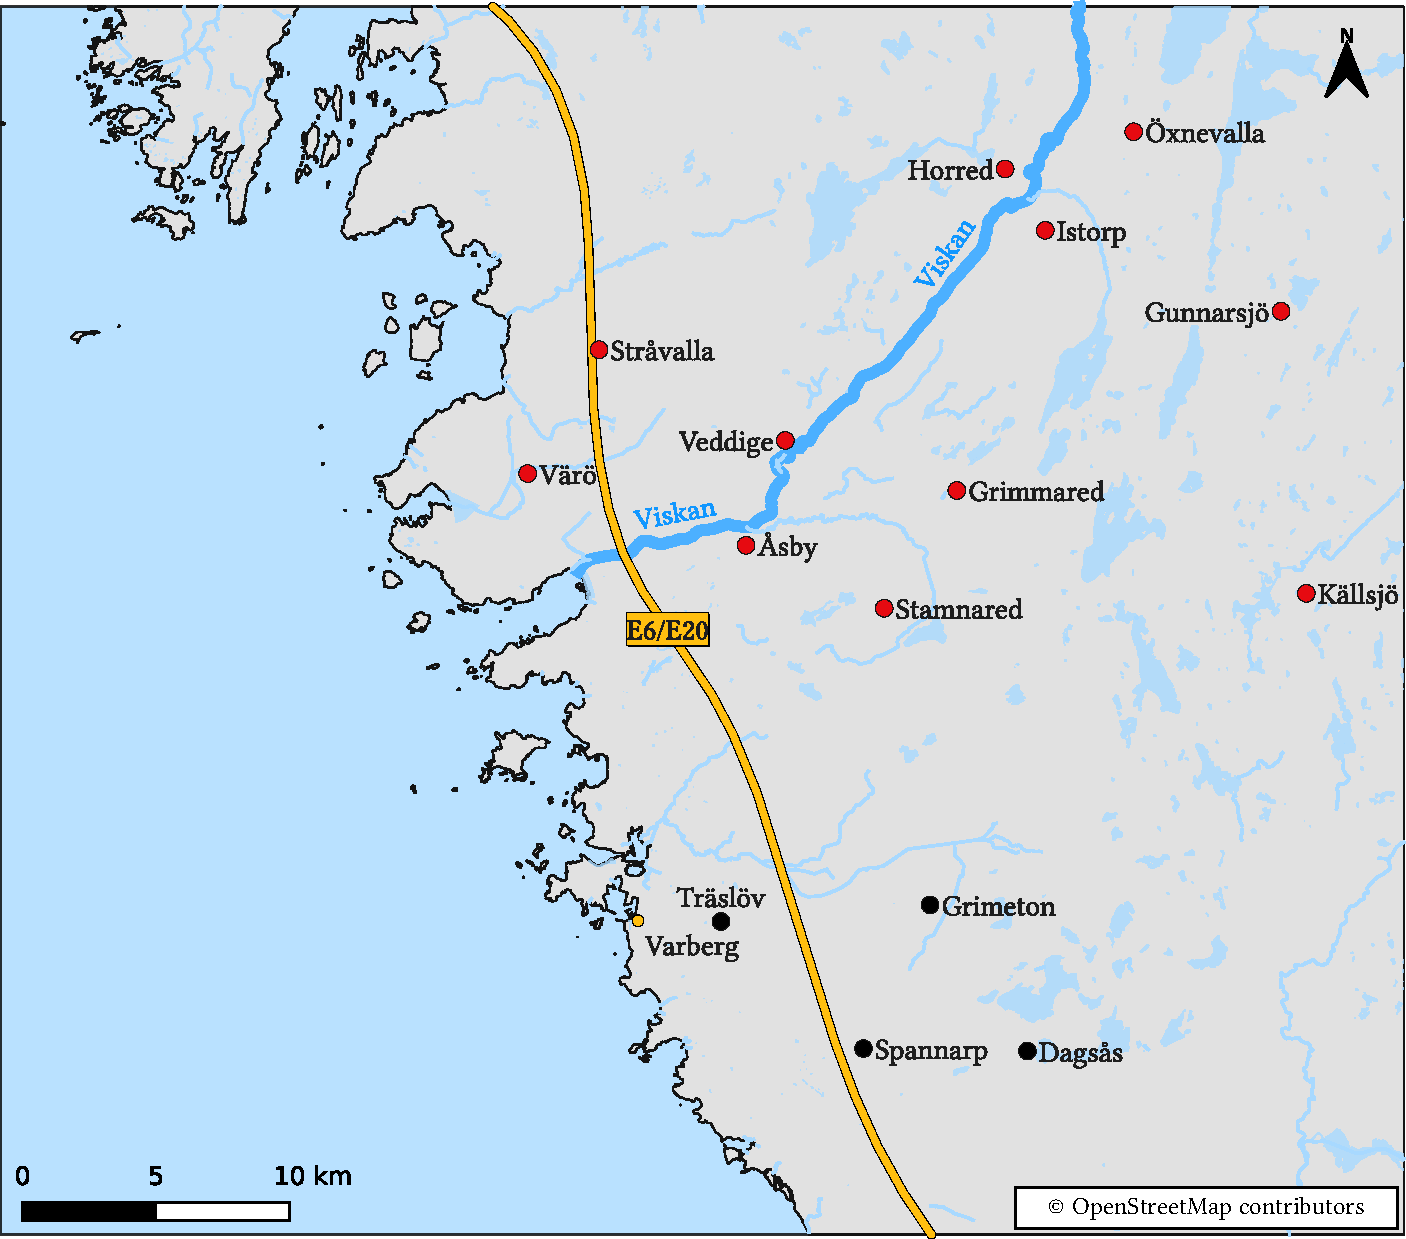
\includegraphics[width=\textwidth]{figures/lmswe-latest-compressed.pdf}
\caption{\label{figmap:petzell:1}\label{figmap:petzell:2}Parishes in central (red) and southern (black) Viskadalen and lower reaches of the River Viskan. Varberg is marked in yellow.}
\end{figure}


Unlike present-day \ili{Standard Swedish}, but like \ili{Old Swedish}, \ili{Viskadalian} exhibits \isi{verbal inflection} for both person and number. For instance, the weak verb ‘read’ has four forms in the present \isi{tense}: \textit{läser} (\textsc{sg}), \textit{läsom} (1\textsc{pl}), \textit{läsen} (2\textsc{pl}), \textit{läsa} (3\textsc{pl}), strikingly reminiscent of the corresponding \ili{Old Swedish} forms \textit{läsir}, \textit{läsum}, \textit{läsin}, \textit{läsa}. Present-day \ili{Standard Swedish} has but one form across the board: \textit{läser}. Now, the so-called \isi{Rich Agreement Hypothesis} (\isi{RAH}) predicts that richly inflected verbs move to the \isi{I-domain}. This means that they should precede \isi{sentence adverbials} in subordinate clauses. On the other hand, uninflected verbs are predicted to remain {in situ} (in \isi{VP}), following \isi{sentence adverbials}. Both present-day \ili{Standard Swedish} (PDS) and \ili{Old Swedish} (OS) behave as expected, given the \isi{RAH}: they display the order Adverbial-Finite verb (AF) and Finite verb-\isi{Adverbial} (FA) respectively, as shown in (\ref{ex:petzell:1a}–b).


\ea\label{ex:petzell:1}
\ea{\label{ex:petzell:1a}
\gll huset    där        vi \textit{gärna} \textit{ville}        bo\\
    house.\textsc{def}  where  we    gladly    want.\textsc{pst}    live.\textsc{inf}  \\}\jambox*{AF (PDS)}
\glt `the house where we would gladly live’  \\
\ex{\label{ex:petzell:1b}
\gll ther      the \textit{mågho} \textit{äy} aff     gånga\\
  where  they    may.3\textsc{pl}    not  off      go.\textsc{inf}\\}\jambox*{FA (OS)}
\glt `from where they must not deviate’ (K-styr)
\z
\z


By contrast, present-day \ili{Viskadalian} appears to falsify the \isi{RAH}: all speakers accept the \isi{AF order}, whereas the \isi{FA order} is judged completely ungrammatical; see (\ref{ex:petzell:2a}–b).\footnote{I have one main informant from Träslövsläge (a man, born in 1955), whom I have consulted on several occasions between 2016 and 2017. In order to verify his own grammaticality \isi{judgements}, he checked many examples (including the two word orders in \REF{ex:petzell:2}) with other fluent \isi{dialect} speakers (in his view).}


\ea\label{ex:petzell:2}
\ea[]{\label{ex:petzell:2a}
\gll De    e           båga        som    vi \textit{inte} \textit{håmm}      lässt        fär.\\
    it      be.\textsc{prs}.\textsc{sg}/3\textsc{pl}  book.\textsc{def}     that    we    not have.\textsc{prs}.1\textsc{pl}  read.\textsc{ptcp}    before\\\jambox*{AF}}
\ex[*]{\label{ex:petzell:2b}
    \gll De  e             båga      som  vi        \textit{håmm}      \textit{inte} lässt        fär.\\
      it      be.\textsc{prs}.\textsc{sg}/3\textsc{pl}    book.\textsc{def}     that  we       have.\textsc{prs}.1\textsc{pl}  not    read.\textsc{ptcp}    before\\\jambox*{*FA}
\glt `it is the book that we have not read before’
}
\z
\z

Going back some generations, however, the \isi{FA order} was indeed a common \isi{subordinate clause} word order in the more central parts of Viskadalen, closer to the river and further from the coast; see \REF{ex:petzell:3a}. However, the \isi{AF order} was the dominant type (see \ref{ex:petzell:3b}).


\ea\label{ex:petzell:3}
\ea{\label{ex:petzell:3a}
\gll mänsker      som \textit{vella} \textit{gärna} pruta\\    
people.\textsc{pl}    that  want.\textsc{prs}.3\textsc{pl}  gladly  bargain.\textsc{inf}\\\jambox*{FA}}
\glt `people that would like to bargain’ (Horr)\footnote{The label within parentheses that accompanies \isi{dialect} examples is an abbreviation of the name of the parish (or in some cases the hundred) where the example was collected. A full description of all sources is given in the Appendix.}  \\
\ex{\label{ex:petzell:3b}
\gll de      da \textit{{inte}} \textit{{kunna}} använna\\
    that    they  not  can.\textsc{prs}.3\textsc{pl}    use.\textsc{inf}\\\jambox*{AF}}
\glt `what they cannot use’ (Värö2)
\z
\z


We know that historically, the \isi{AF order} of today (see \ref{ex:petzell:1a}) is an \isi{innovation} that started spreading over the Scandinavian mainland from the late Middle Ages onwards. By the end of the 17\textsuperscript{th} century, AF had become the dominant order in written \ili{Danish} \citep{Sundquist2003} and Swedish (\citealt{Falk1993}; \citealt{Hakansson2011}); \ili{Norwegian} also seems to follow this pattern (\citealt{Christoffersen1997}; \citealt{Vitterso2004}).\footnote{The diachronic development of \ili{Early Modern Norwegian} is harder to follow than the corresponding development of Swedish and \ili{Danish}. Due to \ili{Danish} rule and linguistic domination, texts in \ili{Norwegian} occur only sporadically up until the 19\textsuperscript{th} century (see \citealt[177–192]{Indrebo2001}).} Clearly, the \isi{AF order} has now spread to present-day southern \ili{Viskadalian}, completely marginalizing the original FA variant (see \ref{ex:petzell:2}). But very recently, the old \isi{FA order} was still in use in central \ili{Viskadalian} (see \ref{ex:petzell:3a}), representing a lingering remnant of a slowly dying medieval speech pattern.



In order to better understand this puzzling variation between FA and AF in Viskadalen, I have conducted a detailed scrutiny of \isi{verbal agreement} in the different \ili{Viskadalian} varieties. There are three important differences between the central and the southern varieties, henceforth labelled CV and SV respectively. Two of them concern the expression of second person: the 2\textsc{sg} morpheme \textit{-(s)t} still exists as an affix in CV but has evolved into a pronoun in SV; 2\textsc{pl} always ends in -\textit{n} in SV, but in CV, the \textit{n} is often missing. Third, the past \isi{tense} stem of the highly frequent verbs \textit{få} ‘get’ and \textit{gå} ‘go’ is the same in the entire paradigm in the south (\textit{fick}-, \textit{gick}-), but varies with number in the central variety (\textsc{sg}: \textit{fick}-, \textit{gick}-; \textsc{pl}: \textit{fing}-, \textit{ging}-).



I will argue that this morphological variation in \ili{Viskadalian} can be neatly accounted for and linked to the word order difference, once we adopt a more fine-grained definition of \isi{agreement} richness than hitherto proposed in the literature. My idea is that we need to keep \isi{semantic richness} and \isi{morphological distinctiveness} separate. Given these two parameters, we can distinguish between 4 types of \isi{agreement}: type 1 (both semantically rich and \isi{morphologically distinct}), type~2 (semantically rich but not \isi{morphologically distinct}), type 3 (\isi{morphologically distinct} but not semantically rich), and type 4 (neither semantically rich nor \isi{morphologically distinct}). I propose that only type 1 \isi{agreement} triggers \isi{V-to-I}.



Although central and southern \ili{Viskadalian} verbs express more or less the same semantic distinctions, it is only in the central variety that \isi{agreement} is \isi{morphologically distinct} (i.e. type 1); in the south, \isi{agreement} instead appears to have been reanalysed as part of \isi{tense} (i.e. developed into type 2). In syntax, this makes all the difference, if one assumes (with \citealt{BobaljikThrainsson1998}) that distinctiveness is a necessary condition for syntactically active \isi{agreement}, triggering \isi{movement} of finite verbs into the \isi{I-domain}. The analysis also predicts the southern development of \textit{(s)t} from affix to pronoun, as well as the loss of number-based stem alternations. 



Moreover, it leaves the ground open for \isi{parallel grammars} in CV, resulting in AF/FA variation (see \ref{ex:petzell:3}). Although \isi{agreement} is always \isi{morphologically distinct} in CV (i.e. type 1 or 3), it is not necessarily semantically rich. With both an \textit{n-}less 2\textsc{pl} and a more sporadic use of \textit{-s(t)}-\isi{inflection}, \isi{agreement} turns to type 3 and ceases to be syntactically relevant (excluding \isi{V-to-I}).



The paper is organized as follows. \sectref{sec:petzell:2} and \sectref{sec:petzell:3} constitute the empirical bulk of the paper: in \sectref{sec:petzell:2}, I present my investigation of FA/AF in \ili{Viskadalian}; in \sectref{sec:petzell:3}, I describe the variation in its verbal morphology, briefly also glancing at the poorer \isi{agreement} found in other varieties in the region. Sections 4–5 are more theoretical: in \sectref{sec:petzell:4}, I discuss the \isi{RAH} in general and the notion of richness in particular; then, in \sectref{sec:petzell:5}, I address the interface between morphology and syntax, and more specifically the syntactic role of \isi{tense} and \isi{agreement} \isi{inflection}. The paper ends with some concluding remarks and remaining questions in \sectref{sec:petzell:6}.


\section{Subordinate clause word order in Viskadalian}\label{sec:petzell:2}


In this section, I investigate the distribution of FA and AF word order in \ili{Viskadalian} subordinate clauses. The section starts with some preliminaries (in \sectref{sec:petzell:2.1}) followed by some notational and methodological points (in §§\ref{sec:petzell:2.2}--\ref{sec:petzell:2.3}), before I present the actual results in \sectref{sec:petzell:2.4}. The findings are summarized and related to the word order in present day Träslövsläge in \sectref{sec:petzell:2.5}.


\subsection{Viskadalen: Area and dialect}\label{sec:petzell:2.1}


For my investigation of \isi{subordinate clause} word order in \ili{Viskadalian}, I have compiled a corpus of audio recordings from the 1940s, 1950s, and 1960s. The recordings were made by regional \isi{dialect} archives in Lund and Uppsala. Today, they are part of the collections of the Institute for Language and Folklore. To be included in the sample, the informants on tape are required to inflect their finite verbs for both person and number consistently throughout the session. I have come across 19 such informants, and this verbal usage is the primary linguistic basis for identifying Viskadalen as a \isi{dialect} area in its own right. In no other variety on the Scandinavian mainland except in north-western \ili{Dalecarlian} (see \citealt{Levander1928}; \citealt{Garbacz2010}, and \sectref{sec:petzell:6} below) do we find archaic morphology of this sort.



Viskadalen stretches over two provinces (Sw. \textit{landskap}), namely Halland and Westrogothia (Sw. \textit{Västergötland}), which is probably why there are surprisingly few attempts to address the variety within traditional dialectology; here, the \isi{dialect} of each province has instead typically been the main objective. Still, from the historical evidence, it is quite clear that Viskadalen has formed an economic unit at least since the Middle Ages, based on the hinterland of the town of Varberg: this is where \ili{Viskadalian} peasants have always traded their agricultural produce (\citealt{Grill1954}: 679; \citealt{Linge1969}: 75–76).



I move on now to the division of \ili{Viskadalian} into two sub-varieties, one central and one southern. In \REF{ex:petzell:4} below, I have specified the names of the parishes within each variety, as well as the number of informants and the total length of the recordings. In \figref{figmap:petzell:1}, I have marked the location of all parishes. As is evident, the two parts of the corpus are neither equally large nor distributed over an equal number of places (or informants). The reason for this is trivial: there are simply no more relevant recordings from the area to include. Nevertheless, the corpora representing the two sub-varieties are sufficiently similar for my present purposes, that is, to investigate the use of AF and FA word order.


\ea\label{ex:petzell:4}
\ea  \ili{Central Viskadalian} – just over 11 hours of recorded speech, 12 informants from 11 parishes (Värö, Stråvalla, Veddige, Åsby, Stamnared, Grimmared, Istorp, Öxnevalla, Gunnarsjö, Källsjö, Horred).  \\
\ex\label{ex:petzell:4b}  \ili{Southern Viskadalian} – almost 10 hours of recorded speech, 7 informants from 4 parishes (Träslöv, Grimeton, Dagsås, Spannarp).
\z
\z


There are both syntactic and morphological reasons for the division of \ili{Viskadalian} into a central and a southern variety. In \sectref{sec:petzell:2.4}, we direct our attention towards the syntactic differences; the morphological differences are the topic of \sectref{sec:petzell:3}.


\subsection{The basic structure of AF and FA order}\label{sec:petzell:2.2}


Since the late 1980s, the standard analysis of the difference between AF and FA in Scandinavian subordinate clauses is that FA reflects \isi{movement} of the finite verb (F) out of \isi{VP} to a position to the left of \isi{sentence adverbials} (A), whereas AF indicates the absence of such \isi{movement}. What specific position the verb ends up in need not concern us yet; for now, I will simply refer to it as I, indicating that it is somewhere in the \isi{I-domain}, at least higher in the syntactic tree than \isi{sentence adverbials}, which are assumed to reside directly to the left of \isi{VP}.\footnote{Similarily, I take “\isi{V in situ}” to mean that V is somewhere in the V-domain.} The difference between AF and FA is shown in (\ref{ex:petzell:5a}–b).


\ea\label{ex:petzell:5}
\ea\label{ex:petzell:5a}
[\textsubscript{IP} \textit{F}\textsubscript{v} [\textsubscript{AdvP} \textit{A} [\textsubscript{VP} t\textsubscript{v}]]]                      \jambox*{\isi{V-to-I} (\isi{FA order})}
\ex\label{ex:petzell:5b}{}  [\textsubscript{AdvP} \textit{A} [\textsubscript{VP} \textit{F}]]                        \jambox*{\isi{V in situ} (\isi{AF order})}
\z
\z


As is well known, all Scandinavian languages are V2 languages. This means that the finite verb always moves to C in main clauses, where it is preceded only by whatever phrase ends up in spec-\isi{CP}. If the subject is clause initial, we get \isi{FA order}, as I show with the \ili{Standard Swedish} example in \REF{ex:petzell:6a}. When something else is topicalized, the subject instead remains in the \isi{I-domain}, thus intervening between F and A (see \ref{ex:petzell:6b}).


\ea\label{ex:petzell:6}
\ea{\label{ex:petzell:6a}
\gll [\textsubscript{CP} Han  \textit{{ville}}\textsubscript{v} [\textsubscript{IP} \textit{{gärna}} t\textsubscript{v}    äta    den]]\\
     ~                   he  want.\textsc{pst}                   ~                  gladly           ~                     eat.\textsc{inf}  it\\}\jambox*{ \isi{V-to-C} ({FA})}
\glt `he would gladly eat it’  \\
\ex{\label{ex:petzell:6b}
\gll [\textsubscript{CP} Den \textit{{ville}}\textsubscript{v} [\textsubscript{IP} han \textit{{gärna}} t\textsubscript{v}    äta]]             \\
     ~                   it  want.\textsc{pst}                  ~                 he    gladly          ~                     eat.\textsc{inf}\\}\jambox*{\isi{V-to-C} (XFSA)}
\glt `he would gladly eat it’
\z
\z


Normally, \isi{V-to-C} \isi{movement} does not occur in subordinate clauses, where C instead hosts a \isi{complementizer}; see \REF{ex:petzell:7a} below. Since \isi{V-to-I} is not an option, \isi{FA order} is out, as can be seen in \REF{ex:petzell:7b}.\largerpage


\ea\label{ex:petzell:7}
\ea[]{\label{ex:petzell:7a}
\gll Den mat [\textsubscript{CP}  som [\textsubscript{IP}  han   \textit{{gärna}}[\textsubscript{VP} \textit{ville}   äta]]]        fick      vi    kasta.          \\
    the  food   ~   that  ~   he    gladly  want.\textsc{pst}  eat.\textsc{inf}      get.\textsc{pst}    we    throw.\textsc{inf}  \\\jambox*{\isi{V in situ} (AF)}
\glt `The food that he would gladly eat, we had to throw away’}

\ex[*]{\label{ex:petzell:7b}
\gll Den  mat [\textsubscript{CP}  som [\textsubscript{IP}  han \textit{ville}\textsubscript{v}        \textit{gärna}       [\textsubscript{VP} t\textsubscript{v}   äta]]] fick    vi    kasta.\\
         the  food  ~  that  ~  he    want.\textsc{pst}    gladly  ~  ~ eat.\textsc{inf} get.\textsc{pst}  we    throw.\textsc{inf}\\\jambox*{*\isi{V-to-I} (FA)}}
\z
\z


However, in certain contexts, an entire \isi{CP} may be embedded under the \isi{complementizer} \textit{att}, ‘that’.\footnote{Unlike \ili{English} \textit{that}, Swedish \textit{att} never introduces relative clauses. Here, the \isi{complementizer} is instead \textit{som} (as in \ref{ex:petzell:7}).} Consequently, both word orders occurring in \isi{main clause} CPs (i.e. FA in \REF{ex:petzell:6a} and XFSA in \REF{ex:petzell:6b}) sometimes occur in embedded contexts; see (\ref{ex:petzell:8a}–d). As in main clauses, the high position of the finite verb is a result of \isi{V-to-C} \isi{movement}.


\ea\label{ex:petzell:8}
\ea{\label{ex:petzell:8a}
\gll Då   sa      hon [\textsubscript{CP}    att [\textsubscript{CP}  han\\
    then    say.\textsc{pst}  she  ~    that   ~   he         \\}\jambox*{emb. \isi{V-to-C} (FA)}
\gll     \textit{{ville}}\textsubscript{v}  [\textsubscript{IP}       \textit{{gärna}}   t\textsubscript{v}  äta      den.]]]   \\
    want.\textsc{pst}  ~  gladly   ~  eat.\textsc{inf}    it\\
\glt `Then she said that he would gladly eat it.’  \\

\ex{\label{ex:petzell:8b}
\gll De      meddelade [\textsubscript{CP}    att [\textsubscript{CP}     den\\
    they  report.\textsc{pst}    ~  that   ~   it          \\}\jambox*{emb. \isi{V-to-C} (XFSA)}
\gll     \textit{{ville}}\textsubscript{v} [\textsubscript{IP} han \textit{{gärna}}    t\textsubscript{v}   äta.]]]    \\
    want.\textsc{pst} ~  he      gladly   ~    eat.\textsc{inf}\\
\glt `They reported that he would gladly eat it.’  \\

\ex{\label{ex:petzell:8c}
\gll Poängen  är     [\textsubscript{CP}  att     [\textsubscript{CP}  han\\
    point.\textsc{def}   is   ~    that   ~    he  \\}\jambox*{emb. \isi{V-to-C} ({FA})}

\gll     \textit{{ska}}\textsubscript{v}      [\textsubscript{IP} \textit{{alltså}}  t\textsubscript{v}    ha        den.]]]  \\
    shall     ~     thus   ~    have.\textsc{inf}    it\\
\glt `The point is that he is supposed to have it, you know.’  \\

\ex{\label{ex:petzell:8d}
\gll Vi    drog      slutsatsen [\textsubscript{CP}    att [\textsubscript{CP}     den\\
    we    draw.\textsc{pst}  conclusion.\textsc{def} ~ that    ~   it   \\}\jambox*{emb. \isi{V-to-C} (XFSA)}

\gll     \textit{{fick}}\textsubscript{v} [\textsubscript{IP}  vi    \textit{{nog}} t\textsubscript{v}     ta      hand  om    sedan.]]]  \\
    get.\textsc{pst} ~ we    probably ~ take.\textsc{inf}  hand   about    later\\
\glt `We came to the conclusion that we would probably have to   \\
    deal with that later.’
\z
\z


Embedded \isi{V-to-C} is possible when the content of the \isi{embedded clause} can be interpreted as asserted by the \isi{speaker} \citep[21]{Andersson1975}. This means either the actual \isi{speaker} as in (\ref{ex:petzell:8c}–d), where it is the person uttering the sentences who asserts the content of the \isi{embedded clause}, or that there is an implicit \isi{speaker} as in (\ref{ex:petzell:8a}–b), where the third person subject of the matrix verb (\textit{hon} ‘she’ in \REF{ex:petzell:8a} and \textit{de} ‘they’ in \REF{ex:petzell:8b}) is reported as having asserted the content of the \isi{embedded clause}. \citet[164–167]{Julien2015} notes that it is not always possible to determine whether the embedded \isi{assertion} is direct or indirect. However, the crucial point remains the same: \isi{speaker} \isi{assertion} (of some sort) appears to be a prerequisite for embedded \isi{V-to-C}.\largerpage



Typically, embedded assertions are the \isi{complement} of some sort of \textit{verbum dicendi} (see ‘say’ and ‘report’ in (\ref{ex:petzell:8a}–b)) or of a semantically equivalent predicate (such as ‘the point is’ in \REF{ex:petzell:8c} and ‘we came to the conclusion’ in \REF{ex:petzell:8d}). As argued by \citet{Julien2009}, the latter type may come in a variety of guises. Minimally, the matrix predicate consists of a single word, for instance the \isi{predicative} \isi{adjective} in an elliptic copular construction (see \ref{ex:petzell:9a} below), the additive \isi{adverbial} \textit{plus} \REF{ex:petzell:9b}, or even an isolated conjunction, such as the adversative \textit{men} in \REF{ex:petzell:9c} (see \citealt{Lyngfelt2003} for more examples).


\ea\label{ex:petzell:9}
\ea{\label{ex:petzell:9a}
\gll (Det  är)         klart [\textsubscript{CP}  att [\textsubscript{CP}  då      \textit{{blir}}\textsubscript{v}\\
    it        be.\textsc{prs}    clear ~   that ~   then  become.\textsc{prs}      \\}\jambox*{emb. \isi{V-to-C} (XFSA)}

\gll     [\textsubscript{IP}    man   \textit{{ju}} t\textsubscript{v}       ledsen.]]]  \\
        ~   one     of\_course ~  sad.\\
\glt `Of course, then you become sad.’  \\

\ex{\label{ex:petzell:9b}
\gll Valparna    är      för    små                   \\
    puppy.\textsc{pl}.\textsc{def}  be.\textsc{prs}  too  small    \\}\jambox*{emb. \isi{V-to-C} ({FA})}
\gll     för    transport.  Plus  [\textsubscript{CP}  att      [\textsubscript{CP}  de\\
    for    transport.  plus   ~ that   ~   they     \\
\gll     \textit{{är}}\textsubscript{v} [\textsubscript{IP}    \textit{{knappast}} t\textsubscript{v}   rumsrena      än.]]]  \\
    be.\textsc{prs}  ~  hardly  ~     housebroken    yet\\
\glt `The puppies are too small to be transported.   \\
    Also, they are hardly housebroken yet.’  \\

\ex{\label{ex:petzell:9c}
\gll Jag    har       köpt       ett  halsband             \\
    I        have.\textsc{prs}  buy.\textsc{ptcp}  a  necklace      \\}\jambox*{emb. \isi{V-to-C} ({FA}) }

\gll     till    Kalle.  Men [\textsubscript{CP}  att [\textsubscript{CP}  jag  \textit{{vet}}\textsubscript{v} [\textsubscript{IP}    \textit{{inte}} t\textsubscript{v}   \\
    to    K    but   ~ that  ~  I    know.\textsc{prs} ~ not ~ \\
\gll     om      han  gillar      det.]]]  \\
    whether  he    like.\textsc{prs}    it\\
\glt `I have bought Kalle a necklace. However, I do not   \\
    know if he will like it.’
\z
\z\largerpage[2]


Furthermore, embedded assertions can also occur in \textit{att} clauses expressing causal, consecutive, or causative meaning (\citealt{Julien2015}: 166–167). This is shown in the examples in \REF{ex:petzell:10}.\footnote{\citet[467]{TelemanEtAl1999} claim
 that \isi{concessive} clauses introduced by \textit{fast(än) att} belong to this group as well. However, according to my native intuitions, \textit{fast att} can only introduce a clause displaying \isi{main clause} word order when it has adversative meaning. Consequently, to me, the second sentence in
 (ia) is parallel with the second sentence in \REF{ex:petzell:9c}. Conversely, in
 (ib), the \isi{AF order} forces a \isi{concessive} meaning, which is infelicitous in this context (hence the \#), since it implies that my lack of knowledge of his preferences is expected to have an impact on his inclination towards pursuing higher education.

    \ea
    \ea[]{
    \gll Han  pluggar    på    universitetet.    Fast      att jag  \textit{vet}  \textit{inte}  om      han  gillar      det.\\
    he    study.\textsc{prs}  on    university.\textsc{def}  although    that    I    know.\textsc{prs}    not    whether  he  like.\textsc{prs}    it \\
    \glt ‘He studies at university. However, I do not know if he likes it.’}
    \ex[\#]{Han pluggar på universitet, fast att jag \textit{inte} \textit{vet} om han gillar det.}
    \z
    \zlast} 


\ea\label{ex:petzell:10}
\ea{\label{ex:petzell:10a}
\gll Anna   gick    hem                               \\
    Anna        went  home    \\}\jambox*{emb. \isi{V-to-C} (XFSA)}

\gll     [\textsubscript{CP}   därför     att [\textsubscript{CP}   så    \textit{{ville}}\textsubscript{v} [\textsubscript{IP} hon   \\
          ~ because  that  ~  so    want.\textsc{pst} ~ she  \\
\gll     \textit{{inte}} t\textsubscript{v}    bli         behandlad.]]]  \\
    not    ~    become.\textsc{inf}    treat.\textsc{ptcp}\\
\glt `Anna went home, because she did not want   \\
    to be treated like that.’

\ex{\label{ex:petzell:10b}
\gll Hon  blev         så  arg [\textsubscript{CP} att [\textsubscript{CP}  hon           \\
    she    become.\textsc{pst}    so  angry ~   that  ~  she  \\}\jambox*{emb. \isi{V-to-C} ({FA})}

\gll     \textit{{skällde}}\textsubscript{v} [\textsubscript{IP} \textit{{helt}} \textit{{enkelt}} t\textsubscript{v}  ut    honom.]]]  \\
    scold.\textsc{pst} ~ whole simple ~  out  him\\
\glt `She was so angry that she simply scolded him.’  \\

\ex{\label{ex:petzell:10c}
\gll Det    innebar    till    slut                         \\
    it      mean.\textsc{pst}  to    end  \\}\jambox*{emb. \isi{V-to-C} ({FA})}

\gll     [\textsubscript{CP}    att [\textsubscript{CP}  jag  \textit{{blev}}\textsubscript{v} [\textsubscript{IP}      \textit{{faktiskt}}  t\textsubscript{v}     \\
          ~ that   ~ I    become.\textsc{pst}   ~ actually ~ \\
\gll     instängd.]]]  \\
    trap.\textsc{ptcp}\\
\glt `In the end, I was actually trapped.’
\z
\z


In sum, subordinate clauses with \isi{FA order} are possible in \ili{Standard Swedish}, but only as instances of embedded \isi{V-to-C} (see \ref{ex:petzell:8a},c, \ref{ex:petzell:9b}–c, \ref{ex:petzell:10b}–c). This is possible in \textit{att} clauses, where the content can be interpreted as asserted by the \isi{speaker} (actual or implicit). In other subordinate clauses, the \isi{complementizer} does not take a \isi{CP} \isi{complement}. Consequently, the \isi{FA order} is ungrammatical, since the syntactic operation creating FA below C, namely \isi{V-to-I} \isi{movement}, is not available (see \ref{ex:petzell:7b}).


\subsection{The word order categories AF and FA}\label{sec:petzell:2.3}


Before proceeding to the distribution of AF and FA in the corpus, a brief methodological point is in order. I have only counted an example as a case of AF if there is an explicit subject preceding this string (i.e. SAF). Without a subject, it is difficult to exclude that the A of the AF string is, in fact, in the higher position for adverbials that we have in examples like \REF{ex:petzell:11} below. Here, A precedes the subject (S), which means that A can tell us nothing of the position of the finite verb.


\ea{\label{ex:petzell:11}
\gll naur  \textit{{inte}} \textit{{vi}}    fiskam\\
when    not  we  fish.\textsc{pst}.1\textsc{pl}\\}\jambox*{{AS}}
\glt `when we were not fishing’ (Träsl1)
\z

As for the FA category, the presence or absence of a subject is irrelevant. However, what follows the FA string can be of relevance; see \REF{ex:petzell:12}, where A is followed by a non-finite verb.


\ea{\label{ex:petzell:12}
\gll om  ja \textit{{hade}} \textit{{bare}} hört\\
if    I         have.\textsc{pst}.\textsc{sg}/3\textsc{pl}  only  hear.\textsc{ptcp}\\}\jambox*{{FA}}
\glt `if only I had been a hearing person’ (Grimm)
\z


If the non-finite verb marks the left edge of the \isi{VP}, A must be to the left of \isi{VP} and the finite verb, in turn, must have moved out of \isi{VP}. As will be evident shortly, however, this diagnostic is valid in \ili{Viskadalian} only for \isi{sentence adverbials}.


\subsection{Results}\label{sec:petzell:2.4}


Let us now consider the use of AF and FA in the corpus. In \tabref{tab:petzell:1a}, I give the numbers for SV in the first row and the numbers for CV in the second row. Although the total number of relevant examples is much greater in CV, the overall tendency is quite clear: \isi{AF order} occurs in both varieties; FA, on the other hand is common in CV, but strikingly marginal in SV.


\begin{table}
\begin{tabular}{lrrrrr}
\lsptoprule
& AF & AF\% & FA & FA\% & Total\\\midrule
SV & 16 & 80\% & 4 & 20\% & 20\\
CV & 42 & 55\% & 34 & 45\% & 76\\
\lspbottomrule
\end{tabular}
\caption{\label{tab:petzell:1a}AF and FA order in Viskadalian subordinate clauses}
\end{table}

\begin{table}
\caption{\label{tab:petzell:1b}Type of FA order}
\begin{tabular}{lrrr}
\lsptoprule
& FA-OK & *FA1 & *FA2\\\midrule
SV & 2 & 0 & 2\\
CV & 17 & 13 & 4\\
\lspbottomrule
\end{tabular}
\end{table}



The difference between the varieties regarding FA becomes even clearer when we consider the nature of the FA cases in more detail; see \tabref{tab:petzell:1b}. Here, I have divided all FA examples into three groups. The first group contains FA examples that would be acceptable in \ili{Standard Swedish} as cases of embedded \isi{V-to-C} (see (8–10) above; hence the label FA-OK). These are introduced by \textit{att} ‘that’, and they can all be interpreted as asserted by the \isi{speaker} (actual or implicit). All but one of the FA-OK examples are embedded under a \textit{verbum dicendi} or a similar matrix; see (\ref{ex:petzell:13a}–b) below; cf. the examples in \REF{ex:petzell:8} above. The remaining one is the causal example given in \REF{ex:petzell:13c}; cf. \REF{ex:petzell:10a}.


\ea\label{ex:petzell:13}
\ea{\label{ex:petzell:13a}
\gll ja  glömde  å    tala          ôm  att      garnet        \\
    I    forget.\textsc{pst}  to    speak.\textsc{inf}    of  that  yarn.\textsc{def}\\}\jambox*{{FA}-OK}

\gll    \textit{{skulle}} \textit{{ju}}        spelltas    \\
    shall.\textsc{pst.sg}/3\textsc{pl}  of\_course  coil.\textsc{inf}.\textsc{pass}\\
\glt `I forgot to tell you that the yarn should of course be coiled' (Värö3)  \\

\ex{\label{ex:petzell:13b}
\gll de    kôm        skrivelse    ifrå  kunglia  majestät           \\
    it    come.\textsc{pst}.\textsc{sg}  decree    from  royal    majesty  \\}\jambox*{{FA}-OK}

\gll    att      da \textit{{få}} \textit{{aldri}} ta=t        \\
    that    they    must.\textsc{prs}.3\textsc{pl}  never    take.\textsc{inf}=it    \\
\glt `there came a royal decree stating that they must never take it’ (Öxn)    \\

\ex{\label{ex:petzell:13c}
\gll för    de   att    da \textit{kunne}       \textit{ente}   manövrera\\
    for    that  that  they  can.\textsc{pst.sg}/3\textsc{pl}  not  navigate.\textsc{inf}\\}\jambox*{{FA}-OK}
\glt `because they could not navigate’ (Träsl1)
\z
\z

The two other FA groups, on the other hand, both contain examples that would be ungrammatical in \ili{Standard Swedish} (hence the *; the numbers following it will be explained shortly). These include restrictive relative clauses (see \ref{ex:petzell:14a} below) and various \isi{adverbial} clauses (e.g. temporal as in \REF{ex:petzell:14b} and \isi{conditional} as in \REF{ex:petzell:14c}).


\ea\label{ex:petzell:14}
\ea{\label{ex:petzell:14a}
\gll da    som \textit{{vöre}} \textit{{då}} lite  försiktiare   \\
    they    that  be.\textsc{pst}.3\textsc{pl}  then    slightly   cautious.\textsc{comp}\\\jambox*{*{FA}2}
\glt `those who were then a bit more cautious’ (Vedd)}

\ex{\label{ex:petzell:14b}
\gll då      svina      \textit{kômme}      \textit{väl}   bôrt                 \\
    when  pig.\textsc{pl}.\textsc{def}  come.\textsc{pst}.3\textsc{pl}  expectedly  away \\}\jambox*{*{FA}1}
\glt `once the pigs got away’ (Värö3)

\ex{\label{ex:petzell:14c}
\gll om  ja \textit{{finge}} \textit{{bara}} kômma    dit            \\
    if    I    get.\textsc{pst}.\textsc{sbjv.sg}/3\textsc{pl}  only  come.\textsc{inf}  there\\}\jambox*{*{FA}1}
\glt `if only I would get to come there’ (Ist)
\z
\z


Three of the *FA examples are introduced by \textit{att}; see \REF{ex:petzell:15} below. However, they cannot be interpreted as CPs conveying an embedded \isi{assertion}: in \REF{ex:petzell:15a}, the \textit{att} clause is the \isi{complement} of a non-assertive matrix verb (‘not remember’), and in \REF{ex:petzell:15b} the semantics of the clause (expressing a purpose) is incompatible with \isi{assertion}. Finally, in \REF{ex:petzell:15c}, the \textit{att} clause is certainly the \isi{complement} of the verb ‘say’, just like many of the FA-OK examples. Still, the \isi{FA order} in \REF{ex:petzell:15c} hardly reflects \isi{V-to-C} \isi{movement}. The reason for this is that the object of the verb \textit{gör}, ‘do.\textsc{prs}.\textsc{sg}’, (i.e. \textit{de}, ‘that’) has been extracted from the \isi{embedded clause} and topicalized in the matrix clause. At least since \citet{Holmberg1986}, we have known that this sort of extraction is incompatible with embedded \isi{V-to-C}, as shown in \REF{ex:petzell:16a} below; cf. the \isi{AF order} in \REF{ex:petzell:16b} where extraction works fine. In effect, the \isi{FA order} in \REF{ex:petzell:15c} cannot be the result of \isi{V-to-C}.


\ea\label{ex:petzell:15}
\ea{\label{ex:petzell:15a}
\gll de    hugar                ja  inte  att    vi              \\
    that      remember.\textsc{prs}.\textsc{sg}  I    not    that  we   \\}\jambox*{*{FA}1}

\gll \textit{ådem} \textit{särskilt}      gröd   \\
     eat.\textsc{pst}.1\textsc{pl}    particularly    porridge\\
\glt `I cannot remember that there was a particular tradition for us to have porridge’ (Strå)  \\

\ex{\label{ex:petzell:15b}
\gll för      att    de \textit{{skulle}} \textit{{säkert}} vara                                         värme    nock   \\
    for      that  it    shall.\textsc{pst.sg}/3\textsc{pl}    surely  be.\textsc{inf}  heat      enough\\\jambox*{*{FA}1}
\glt `in order for it to be sufficiently hot for sure’ (Strå)}

\ex{\label{ex:petzell:15c}
\gll de\textsubscript{i}      sa          ja  att    ja \textit{{gör}}      \textit{{inte}} t\textsubscript{i}\\
    that    say.\textsc{pst}.\textsc{sg}    I  that  I    do.\textsc{prs}.\textsc{sg}     not  \\}\jambox*{*{FA}1}
\glt `I said that I will not do that’ (Ist)
\z
\z

\ea\label{ex:petzell:16}
\ea[*]{\label{ex:petzell:16a}
\gll Den\textsubscript{i}  trodde      jag  att    du \textit{{hade}} \textit{{faktiskt}}\\
     that      think.\textsc{pst}  I    that  you have.\textsc{pst}    actually\\\jambox*{emb. \isi{V-to-C} ({FA})}
\gll sett t\textsubscript{i}\\
     seen\\}
    

\ex[]{\label{ex:petzell:16b}
\gll Den\textsubscript{i}   trodde    jag  att    du   \textit{{faktiskt}} \textit{{hade}} sett t\textsubscript{i}\\
    that      think.\textsc{pst}  I    that  you  actually    have.\textsc{pst}    seen\\\jambox*{\isi{V in situ} ({AF})}
\glt `I thought that you had actually seen it’}
\z
\z


I move on now to the difference between *FA1 and *FA2, which regards the nature of A. In the former group, the A is a sentence \isi{adverbial} (including negation); see (\ref{ex:petzell:17a}–b) below (as well as (\ref{ex:petzell:14b}–c) and \REF{ex:petzell:15} above).\footnote{These are the particular adverbials that occur in the 13 *FA1 examples: 3 \textit{la} `presumably’, 2 \textit{inte} ‘not’, 2 \textit{bara} ‘just’, 1 \textit{gärna} ‘gladly’, 1 \textit{eventuellt} ‘possibly’, 1 \textit{säkert} ‘surely’, 1 \textit{särskilt} ‘particularly’, 1 \textit{väl} ‘expectedly’, 1 \textit{kanske} ‘maybe’.} By contrast, the *FA2 adverbials are all temporal, as in (\ref{ex:petzell:17c}–d) (see also \ref{ex:petzell:14a}).{}


\ea\label{ex:petzell:17}
\ea{\label{ex:petzell:17a}
\gll den  förlusta    vi \textit{{skullem}}    \textit{{eventuellt}}    lia\\
    the      loss.\textsc{def}    we    shall.\textsc{pst}.1\textsc{pl}  possibly  suffer.\textsc{inf}\\\jambox*{*{FA}1}
\glt  `the loss we would possibly suffer’ (Ås)}

\ex{\label{ex:petzell:17b}
\gll de    va      en  gang  som    ja  \textit{{åkte}} \textit{{inte}}    te  gästis\\
    it    be.\textsc{pst}.\textsc{sg}  a  time  that    I  travel.\textsc{pst.sg}/3\textsc{pl}  not    to  inn\\\jambox*{*{FA}1}
\glt `it was a time that I did not go to the inn’ (Ist)}

\ex{\label{ex:petzell:17c}
\gll {om\textsubscript{}} de \textit{{va}} \textit{{nu}} laom    tört\\
    if    it    be.\textsc{prs}.\textsc{sg}  now  just    dry  \\\jambox*{*{FA}2}
\glt   `if it was dry enough now’ (Spann)}
\ex{\label{ex:petzell:17d}
\gll när    da \textit{{hade}} \textit{{då}} slått=et\\
    when  they  have.\textsc{pst.sg}/3\textsc{pl}  then  beat.\textsc{ptcp}=it\\\jambox*{*{FA}2}
\glt `when they had then beaten it (i.e. the hay)’ (Vedd)}
\z
\z


\isi{Temporal adverbials} may certainly occur in the same position as \isi{sentence adverbials}, directly to the left of \isi{VP}, as can be seen in the AF example in \REF{ex:petzell:18a} below. However, in \ili{Viskadalian}, \isi{temporal adverbials} could also reside in a medial \isi{VP} position, after the finite verb but before complements of the verb. We see this in \REF{ex:petzell:18b}. Here, the finite verb is clearly in situ, since it is preceded by the sentence \isi{adverbial} \textit{liaväl}. The PP \textit{om viskepelser} is an \isi{adverbial} argument occupying a \isi{complement} position somewhere below V\textsuperscript{o}. Consequently, the intervening \textit{nu} must be somewhere in \isi{VP}.


\ea\label{ex:petzell:18}
\ea{\label{ex:petzell:18a}
\gll när    da \textit{{då}} \textit{{komme}} ain    bit                \\
    when    they  then  come.\textsc{pst}.3\textsc{pl}    a     piece\\}\jambox*{{AF}}
\glt `when they then made some progress’ (Värö3)
\ex{\label{ex:petzell:18b}
\gll eftersom    vi \textit{{liaväl}} \textit{{pratam}} \textit{{nu}}   om      viskepelser   \\
    since      we    anyway    talk.\textsc{pst}.1\textsc{pl}  now        about    superstition.\textsc{pl}\\\jambox*{{AFA}}    
\glt `since we were just talking about superstitions anyway’ (Träsl2)}
\z
\z


Given that \isi{temporal adverbials} can appear within \isi{VP} (as in \ref{ex:petzell:18b}), we cannot exclude that the A has precisely that position in FA examples like \REF{ex:petzell:14a} and (\ref{ex:petzell:17c}–d). In that case, the reason that these examples are bad in \ili{Standard Swedish} is that \ili{Standard Swedish} is not as liberal when it comes to VP-medial placement of \isi{temporal adverbials} as \ili{Viskadalian} is. For the*FA1-type, on the other hand, such an explanation is not available, since \isi{sentence adverbials} never appear as the second \isi{adverbial} in AFA strings like \REF{ex:petzell:18b}.\footnote{One
    reviewer suggests that the lack of examples where the lower \isi{adverbial} is a sentence \isi{adverbial} might be because the sentence \isi{adverbial} needs to take scope over the higher \isi{adverbial}. If this were the case, we would expect the restriction to be at work also when both adverbials precede the finite verb, which they do in \ili{Standard Swedish}. However, both orders are possible in the standard equivalent to \REF{ex:petzell:18b}; see (ia–b). In fact, the one where the sentence \isi{adverbial} (\textit{ändå}) does not take scope over the temporal (\textit{nu}) \isi{adverbial} feels more natural than the alternative order (as indicated by the single \isi{question} mark in (ib)). This strongly suggests that the lack of post-finite \isi{sentence adverbials} in clauses with AFA word order has a syntactic rather than a semantic explanation.
    \ea
    \ea[]{
    \gll eftersom  vi \textit{{nu}} \textit{{ändå}} pratade  om    vidskepelser\\
    since        we  now  anyway  talk.\textsc{pst}  about  superstition.\textsc{pl}\\
    }
    \ex[?]{eftersom vi \textit{{ändå}} \textit{nu} pratade om vidskepelser
    \glt  ‘since we were just talking about superstitions anyway’
    }
    \z
    \z
}
Consequently, the only reasonable way to explain the 13 instances of *FA1 order in CV is to conclude that \isi{V-to-I} was indeed possible in this variety.\footnote{Many scholars in the past have claimed that only FA clauses with \isi{sentential negation} are unambiguous indicators of \isi{V-to-I} \isi{movement}, since \isi{sentential negation} (unlike other adverbials) has to appear above \isi{VP} (\citealt{Falk1993}: 171–172; \citealt{WiklundEtAl2007}: 222–223; \citealt{KoenemanZeijlstra2014}: 586; \citealt{HeycockSundquist2017}: 177–178). However, such rigidity is hardly called for in my \ili{Viskadalian} sample. Here, all \isi{sentence adverbials} refuse to appear as the second \isi{adverbial} in AFA contexts, indicating that they are all unable to reside in \isi{VP} and thereby – when appearing to the right of the finite verb (i.e. FA) – constitute solid indicators of verb \isi{movement} out of \isi{VP}.}



As pointed out, FA-OK could be the result of \isi{V-to-C} \isi{movement}. However, on such an account, it is hard to understand why FA-OK is so much more common in CV than it is in SV. If we instead assume that it is the possibility of applying \isi{V-to-I} in CV that is responsible for the frequent use of FA-OK, the difference between the varieties follows straightforwardly. See \citet{Falk1993} and \citet{Sundquist2003} for a similar approach to FA-OK in historical Swedish and \ili{Danish}. 



Still, it is evident that \isi{V-to-I} is not mandatory in CV. \isi{AF order} not only occurs in CV, it in fact outnumbers the FA variant. The simplest (and most probable) analysis of AF is that V is in situ, as in \REF{ex:petzell:5b} above. How to account for this variation in CV is the topic of \sectref{sec:petzell:5.3} below.


\subsection{Summary}\label{sec:petzell:2.5}\largerpage[2]


As shown in the introduction (see example \ref{ex:petzell:2}), present day speakers of SV (in Träslövsläge) find the \isi{FA order} derived by \isi{V-to-I} highly ungrammatical. Now, adding the results from the investigation of 20\textsuperscript{th} century \ili{Viskadalian} (south and central), the \isi{judgements} of the modern speakers are hardly surprising: there was no \isi{V-to-I} in SV a couple of generations back either.{} In the recordings from CV, on the other hand, \isi{V-to-I} and \isi{V in situ} occurred side by side.


\section{Verbal morphology in Viskadalian and beyond}\label{sec:petzell:3}


The main aim of this section is to describe the various forms of (indicative) finite verbs in traditional \ili{Viskadalian}; this description is given in \sectref{sec:petzell:3.1}. In \sectref{sec:petzell:3.2}, I broaden the perspective, addressing the less differentiated inflectional systems in the neighbouring dialects. \sectref{sec:petzell:3.3} is a summary.


\subsection{Agreement inflection in traditional Viskadalian}\label{sec:petzell:3.1}


My primary source for the \ili{Viskadalian} \isi{inflectional paradigm} is the same collection of audio recordings used in the word order investigation (see \sectref{sec:petzell:2.1} above). In addition, I have consulted a number of descriptions of the \isi{dialect} of specific parts of Viskadalen. These include (in chronological order): \citet{Moller1858}; \citet{Belfrage1871}; \citet{Andersson1922}; \citet{Kalen1923}; \citet{Lindberg1927}; \citet{GotlindLandtmanson1950}.



To exemplify the full array of varying forms, I use both disyllabic and monosyllabic verbs, both strong verbs and weak verbs, and, finally, both verbs in the present \isi{tense} and verbs in the past \isi{tense}. I give all the present \isi{tense} forms in \tabref{tab:petzell:2a} and all the past \isi{tense} forms in \tabref{tab:petzell:2b}. The hyphen (-) marks the boundary between stem and ending.


\begin{table}
\caption{\label{tab:petzell:2a}Viskadalian present tense inflection}
\fittable{\begin{tabular}{lllllllll}
\lsptoprule
& \multicolumn{2}{c}{‘read’} & \multicolumn{2}{c}{‘begin’} & \multicolumn{2}{c}{‘get’} & \multicolumn{2}{c}{‘have’}\\\cmidrule(lr){2-3}\cmidrule(lr){4-5}\cmidrule(lr){6-7}\cmidrule(lr){8-9}
& CV & SV & CV & SV & CV & SV & CV & SV\\
\midrule
\textsc{1sg} & läs-er & läs-er & börja-r & börja-r & få-r & få-r & ha-r & ha-r\\
\textsc{2sg} & läs-er & läs-er & börja-r & börja-r & få-r & få-r & ha-r/st & ha-r\\
\textsc{3sg} & läs-er & läs-er & börja-r & börja-r & få-r & få-r & ha-r & ha-r\\
\textsc{1pl} & läs-om & läs-om & börj-om & börj-om & få-m & få-m & ha-m & ha-m\\
\textsc{2pl} & läs-e(n) & läs-en & börj-e(n) & börj-en & få-(n) & få-n & ha-(n) & ha-n\\
\textsc{3pl} & läs-a & läs-a & börj-a & börj-a & få & få & ha & ha\\
\lspbottomrule
\end{tabular}}
\end{table}

\begin{table}
\caption{\label{tab:petzell:2b}Viskadalian past tense inflection}
\fittable{\begin{tabular}{lllllllll}
\lsptoprule
& \multicolumn{2}{c}{‘read’} & \multicolumn{2}{c}{‘begin’} & \multicolumn{2}{c}{‘get’} & \multicolumn{2}{c}{‘have’}\\\cmidrule(lr){2-3}\cmidrule(lr){4-5}\cmidrule(lr){6-7}\cmidrule(lr){8-9}
& CV & SV & CV & SV & CV & SV & CV & SV\\
\midrule
\textsc{1sg} & läs-te & läs-te & börja & börja & fick & fick & ha-de & ha-de\\
\textsc{2sg} & läs-te(st) & läs-te & börja-(st) & börja & fick-(st) & fick & ha-de(st) & ha-de\\
\textsc{3sg} & läs-te & läs-te & börja & börja & fick & fick & ha-de & ha-de\\
\textsc{1pl} & läs-tem & läs-tem & börja-m & börja-m & fing-em & fick-em & ha-dem & ha-dem\\
\textsc{2pl} & läs-te(n) & läs-ten & börja-(n) & börja-n & fing-e(n) & fick-en & ha-de(n) & ha-den\\
\textsc{3pl} & läs-te & läs-te & börja & börja & fing-e & fick-e & ha-de & ha-de\\
\lspbottomrule
\end{tabular}}
\end{table}

Let us first address some general issues, starting with the vowel in endings expressing 1\textsc{pl}: the system given in the tables, where there is an \textit{e} in the past \isi{tense} and an \textit{o} in the present \isi{tense}, is the most common in actual speech. There is some variation: \textit{o} appears on occasion in the past \isi{tense} as well, all over Viskadalen, and the pronunciation of \textit{o} is often more \textit{u}-like in the Westrogothian part of CV. What does not exist, however, is the use of \textit{e} in 1\textsc{pl} endings in the present \isi{tense} (*\textit{läsem}).\footnote{In present-day Träslövsläge, the vowel in 1\textsc{pl} is always \textit{o}; this is a recent development that I will not address here.} Another general point regards weak verbs of the \textit{börja} type. Originally, there was a dental affix there as well (\textit{börja}-\textbf{\textit{de}}-\textit{m}), but this is all gone, as can be seen. There is a lingering effect of this affix, though: the final vowel of the past \isi{tense} stem is more robust than the final vowel of the present \isi{tense} stem. Although superficially identical (\textit{börja}), the \textit{a} vowel is intact across the paradigm in the past \isi{tense}, but deleted in the present \isi{tense} when the \isi{agreement} affix starts with a vowel.



Now, there are some important morphological differences between CV and SV. First, the two varieties differ with respect to the expression of second person, both in the plural and the singular. In CV, we still find the old \textit{-(s)t} ending for 2\textsc{sg}.\footnote{In \ili{Old Swedish}, the \textit{s} occurred only when the verb stem ended in \textit{t}/\textit{d} (\textit{bad-st}, ‘pray.\textsc{pst.sg}-\textsc{2sg}’), but during the early modern era, most notably in the \isi{Bible} from 1541, the \textit{s} was used more generally, including with other stem endings (\textit{gaf-st}, \textit{tok-st}, ‘give.\textsc{pst.sg}-2\textsc{sg}, take.\textsc{pst}-\textsc{2sg}’). With stems ending in \textit{l} or \textit{n}, the \textit{s} is never part of the affix, neither in historical texts nor in \ili{Viskadalian}. In the latter case, the stem-final consonant is sometimes suppressed in these contexts, for instance \textit{skal-t} → \textit{ska-t} ‘shall.\textsc{prs.sg}-2\textsc{sg}’.} This ending never co-occurs with the -\textit{r}-ending, which means that it is more common in the past than in the present \isi{tense}. As we can see in \tabref{tab:petzell:1a}, most verbs have the -\textit{r} ending across the singular, ‘have’ being the only exception; with this verb, there is variation between -\textit{r} and -\textit{st} in 2\textsc{sg}. This sort of variation is quite uncommon, and there are only a few similar verbs (e.g. \textit{si\textbf{{st}}} ‘see.\textsc{prs}.2\textsc{sg}’, which varies with \textit{si\textbf{{r}}} ‘see.\textsc{prs}.\textsc{sg}’, and \textit{ä\textbf{{st}}} ‘be.\textsc{prs.}2\textsc{sg}’, which varies with \textit{ä\textbf{{r}}} ‘be.\textsc{prs}.\textsc{sg}’).



Nevertheless, \textit{-(s)t} is by no means banned from the present \isi{tense}, it is only incompatible with -\textit{r}, which, in turn, is restricted to the present \isi{tense}. There are so-called preterite-present verbs that never have the -\textit{r}-ending; consequently, \mbox{-\textit{(s)t}} works fine: \textit{kan\textbf{{t}}} ‘can.\textsc{prs}.2\textsc{sg}’, \textit{ska\textbf{{t}}} ‘shall.\textsc{prs}.2\textsc{sg}’, \textit{vai\textbf{{st}}} ‘know.\textsc{prs.}2\textsc{sg}’. Furthermore, this affix is more versatile in CV than it ever was in \ili{Old Swedish}, most notably since it occurs in the past \isi{tense} of weak verbs (see \textit{läste\textbf{{st}}}, \textit{hade\textbf{{st}}} in the table).



Both the -\textit{(s)t} ending and the -\textit{n} ending for 2\textsc{pl} are somewhat unstable in CV. They are attested all over the area, but they may be inconsistently represented even within the system of a single informant; this motivates the parentheses surrounding them in the table. By contrast, in SV, the -\textit{n} ending is robust, whereas the -\textit{(s)t} ending is completely absent.



Second, the stem in the past \isi{tense} of the highly frequent verbs \textit{få} ‘get’, and \textit{gå} ‘go’ varies with number in CV, but not in SV. This can be seen with the verb \textit{få} in \tabref{tab:petzell:2b}, where SV has the stem \textit{fick-} across the board but CV has \textit{fick-} only with singular subjects and \textit{fing-} with plural subjects.



There are some additional differences between CV and SV regarding pronouns, most of which are simply irrelevant for the issues at hand.\footnote{These include, for instance, the form of the free 3\textsc{pl} pronoun, which is \textit{dai} in SV and \textit{da} in CV, and the form of the 1\textsc{sg} \isi{clitic}, which is \textit{ik} in CV but \textit{ja} in SV (in the latter case coinciding with the free pronoun). For a thorough description and discussion of the \ili{Viskadalian} \isi{pronominal system}, see \citet{Petzell2017}.} One pronominal difference, however, is crucial for our understanding of the \isi{agreement} system in general. It concerns the expression of second person singular and is clearly related to the difference regarding second person \isi{inflection} described above. In CV, the 2\textsc{sg} \isi{clitic} is always \textit{ä}; see \REF{ex:petzell:19}. By contrast, in SV the 2\textsc{sg} \isi{clitic} is either \textit{tä} or \textit{stä}, as shown in \REF{ex:petzell:20}.


\ea\label{ex:petzell:19}
\ea\label{ex:petzell:19a}
\gll töcker=ä \\
    think.\textsc{prs.sg=}ä (Fag)    \\
\ex\label{ex:petzell:19b}
\gll skat=ä   \\
    shall.\textsc{prs}.2\textsc{sg}=ä (G-sjö)  \\
\ex\label{ex:petzell:19c}
\gll vaist=ä   \\
    know.\textsc{prs}.2\textsc{sg}=ä (Värö1)\\
\z
\ex\label{ex:petzell:20}
\ea\label{ex:petzell:20a}
\gll töcker=tä \\
    think.\textsc{prs.sg}=you.sg.cl (Himl)  \\
\ex\label{ex:petzell:20b}
\gll kan=tä   \\
    kan.\textsc{prs.sg}=you.\textsc{sg}.\textsc{cl} (from \citealt{Andersson1922})  \\
\ex\label{ex:petzell:20c}
\gll hade=stä   \\
    have.\textsc{pst}.\textsc{sg}/3\textsc{pl}=you.\textsc{sg}.\textsc{cl} (Dags)\\
\z
\z


Consider, first, the (a) examples, where the verb forms are identical (\textit{töcker}), straightforwardly distinguishing the CV \isi{clitic} \textit{ä} from the SV \isi{clitic} \textit{tä}. However, from the forms in the (b) and (c) examples alone we cannot determine where the verb ends and the \isi{clitic} starts. To be able to conclude that the SV \isi{clitic} is indeed \textit{(s)tä}, we need to rely on the \isi{inflection} paradigm. Seeing that there is never any \isi{inflection} for 2\textsc{sg} with subject-verb word order in SV (*\textit{du kant}, *\textit{du hadest}), the \textit{(s)t} sequences in (\ref{ex:petzell:20b}–c) can hardly be affixes; consequently, they have to belong to the \isi{enclitic pronoun}. As for CV, on the other hand, \textit{(s)t} does function as an affix (e.g. \textit{du skat, du vaist}); thus, we have strong reason to assume that the \isi{clitic} is \textit{ä}, not only in \REF{ex:petzell:19a}, but also in (\ref{ex:petzell:19b}–c).



Now, disregarding second person singular, the enclitic \textit{ä} is by no means restricted to CV. In SV, it occurs both in 1\textsc{pl} and in 2\textsc{pl,} as can be seen in (\ref{ex:petzell:21a}–b). In CV, the usage of \textit{ä} is less consistent in the plural: in 2\textsc{pl}, it only occurs together with the -\textit{n} ending; without it, the inverted subject is the free pronoun; see (\ref{ex:petzell:22a}–a′). However, in 1\textsc{pl}, the \textit{ä} is as robust as in SV (see \ref{ex:petzell:22b}).


\ea\label{ex:petzell:21}
\ea\label{ex:petzell:21a}
\gll ficken=ä \\
    get.\textsc{pst}.2\textsc{pl}=ä (Träsl1)  \\
\ex\label{ex:petzell:21b}
\gll vävom=ä   \\
    weave.\textsc{prs}.1\textsc{pl}=ä (Träsl1)\\
\z
\ex\label{ex:petzell:22}
\ea\label{ex:petzell:22a}
\gll fengen=ä \\
    get.\textsc{pst}.2\textsc{pl}=ä (Värö1)  \\
\exi{a\parbox{0mm}{$'$}.}
\gll skräppe      i\\
    boast.\textsc{prs}.2\textsc{pl}   you.\textsc{pl} (from \citealt{Lindberg1927})  \\
\ex\label{ex:petzell:22b}
\gll gjordem=ä   \\
    do.\textsc{pst}.1\textsc{pl}=ä (Strå)\\
\z
\z


It may seem tempting to analyse the \textit{ä} as some sort of \isi{dummy pronoun}, licensed by semantically rich \isi{agreement}: it does occur when the reference of the subject is explicitly expressed in the ending, as in (\ref{ex:petzell:19b}–c), \REF{ex:petzell:21}, and (\ref{ex:petzell:22a}, b), but it does not occur in 2\textsc{pl} when there is no -\textit{n} (as in \ref{ex:petzell:22}a$'$). The absence of \textit{ä} in (\ref{ex:petzell:22a}′) could possibly be linked to the fact that the remaining ending -\textit{e} does not unambiguously point to a 2\textsc{pl} referent (as further explicated in \sectref{sec:petzell:4.2} below). Such an analysis does not hold, however, when we include examples like \REF{ex:petzell:19a}, where \textit{ä} follows the -\textit{r} ending, which only marks the singular. Furthermore, the \textit{ä} is not compatible with -\textit{a}, although this ending is unique to 3\textsc{pl}.


\subsection{Less richly inflected verbs further to the southeast}\label{sec:petzell:3.2}


In other places to the south and southeast of Viskadalen, the traditional dialects inflect their finite verbs to a varying extent (see \citealt{Horn2015,Horn2017} for details). There are no varieties where there is a distinction between all three persons (as in \ili{Viskadalian}). But south of Viskadalen, we find varieties which make a distinction between 1/2\textsc{pl} on the one hand (expressed with the original -\textit{n} ending for 2\textsc{pl}) and 3\textsc{pl}, as shown in \REF{ex:petzell:23a} below with the verb \textit{få} ‘get’, in the past \isi{tense}. Even further to the south, primarily in the province of Skåne, the -\textit{n} form lived on as a designated 2\textsc{pl} form together with a common 1/3\textsc{pl} ending (originally used for 3\textsc{pl}); see \REF{ex:petzell:23b}. Note that the number-based \isi{stem alternation} found in central (but not southern) \ili{Viskadalian} is \isi{productive} in these less richly inflecting varieties as well.

\ea\label{ex:petzell:23}
\begin{multicols}{2}
\ea \label{ex:petzell:23a}\begin{tabbing}
    1/2\textsc{pl}  \=   \textit{fing-en}  \kill
    \textsc{sg}     \> \textit{fick}\\                          
    1/2\textsc{pl}  \>  \textit{fing-en}\\
    3\textsc{pl}    \>    \textit{fing-e}
    \end{tabbing}
\ex \label{ex:petzell:23b}\begin{tabbing}
   1/3\textsc{pl} \= \textit{fing-e}\kill
   \textsc{sg}    \> \textit{fick}\\
   1/3\textsc{pl} \> \textit{fing-e}\\
   2\textsc{pl}   \> \textit{fing-en}
   \end{tabbing}
\z
\end{multicols}
\z


The most widespread \isi{verbal inflection} in the Swedish southwest, at least when we reach the middle of the 20\textsuperscript{th} century, is \isi{inflection} for number only; see \REF{ex:petzell:24a} below, where the ending for 3\textsc{pl} is generalized to all plural persons. We find this system in the traditional dialects of a vast area, including southern Halland, as well as parts of the provinces of Skåne, Blekinge, and Småland. In a small area in the southeast of Småland (in the parish of Södra Sandsjö, which is outside of \figref{figmap:petzell:1}), there appear to have existed varieties where the original 2\textsc{pl} ending had developed into a general plural; see \REF{ex:petzell:24b}.\footnote{I have not come across the system in \REF{ex:petzell:24b} in any audio recording, nor is it mentioned by \citet{Horn2015,Horn2017}; the only source of it is \citet{Granstrom1915}.}


\ea\label{ex:petzell:24}
\ea\label{ex:petzell:24a}  \textsc{sg}:  \hspace{\tabcolsep}  \textit{fick};  \hspace{2\tabcolsep}    \textsc{pl:} \hspace{\tabcolsep}  \textit{fing-e}
\ex\label{ex:petzell:24b}  \textsc{sg}:  \hspace{\tabcolsep}  \textit{fick};  \hspace{2\tabcolsep}    \textsc{pl:} \hspace{\tabcolsep}  \textit{fing-en}
\z
\z


As can be seen, the \isi{stem alternation} is intact even in the dialects with \isi{inflection} only for number.


\subsection{Summary}\label{sec:petzell:3.3}


This section contains a detailed description of \isi{verbal agreement} in \ili{Viskadalian}, with a specific focus on the differences between the central (CV) and the southern (SV) varieties. In CV, we find both the -\textit{(s)t} affix for 2\textsc{sg} and -\textit{en} for 2\textsc{pl,} but neither of them is used consistently. In SV, by contrast, the -\textit{en} is robust and the \textit{-(s)t} non-existent. There is, however, a remnant of the \textit{-(s)t} affix in the 2\textsc{sg} \isi{clitic}, which is \textit{(s)tä} in SV, not \textit{ä} as in CV. Furthermore, the past \isi{tense} stem form of \textit{få}/\textit{gå} varies with number in CV, but not in SV. Such stem variation is also found in neighbouring dialects where verbs are less richly inflected than in Viskadalen.


\section{The Rich Agreement Hypothesis }\label{sec:petzell:4}


This section starts with an overview of the \isi{RAH} in \sectref{sec:petzell:4.1}, from its birth in the 1980s to its present day status. Then, in \sectref{sec:petzell:4.2}, I present my two-dimensional definition of rich \isi{agreement}. In \sectref{sec:petzell:4.3}, I address the difference between CV and SV, and propose a way to derive it diachronically. \sectref{sec:petzell:4.4} is a summary.


\subsection{The history of the Rich Agreement Hypothesis: Birth, life, death, and resurrection}\label{sec:petzell:4.1}
\begin{sloppypar}
At least since the mid-1980s, the empirical correlation between \isi{agreement} and the position of finite verbs in the Scandinavian languages has fascinated researchers. \citet{Kosmeijer1986} set the ball in motion by drawing attention to the word order difference in subordinate clauses between \ili{Icelandic} (\isi{FA order}) and \ili{Mainland Scandinavian} (\isi{AF order}), proposing that this difference was grammatically linked to the presence (\ili{Icelandic}) and absence (\ili{Mainland Scandinavian}) of \isi{verbal agreement}. Although this presumed link, later labelled the \isi{Rich Agreement Hypothesis} (\isi{RAH}), was explored early on in the history of Swedish as well by \citet{Platzack1988emergence}, the early to mid-1990s were the prime era for the \isi{RAH}. It inspired many of the (now classic) monographs on \ili{Germanic} morphosyntax that were published during this period (e.g. \citealt{Falk1993}; \citealt{Rohrbacher1994}; \citealt{Vikner1994}; \citealt{HolmbergPlatzack1995}). 
\end{sloppypar}


However, by the turn of the new millennium, the \isi{RAH} appears to have lost its appeal: more and more exceptions turned up, forcing the formulation of a weaker (and less interesting) hypothesis (see \citealt{BobaljikThrainsson1998} and \citealt{Sundquist2003} for discussion). Some even suggested that the \isi{RAH} be abandoned altogether \citep{WiklundEtAl2007}. Still, the \isi{RAH} did not die. A few years ago, it was defended by \citet{KoenemanZeijlstra2014}, who argue that it should be rehabilitated in its strongest form (having rejected all known counter-evidence). And even more recently, in 2017, Tvica entered the scene with his dissertation \citep{Tvica2017}, in which, unlike previous studies of rich \isi{agreement} and word order, he tests the \isi{RAH} on a typologically balanced sample. Hitherto, the empirical scope has been limited to \ili{Germanic}, with few exceptions, and to \ili{Indo-European} with no exceptions (to my knowledge). In contrast, Tvica’s sample consists of 24 languages that are neither related to each other nor belong to the \ili{Indo-European} family. Given that the \isi{RAH} has never been tested this thoroughly before, the outcome of Tvica’s study will, no doubt, be a natural starting point for all future testing of the hypothesis. 



Among Tvica’s 24 languages, there are 17 that corroborate the \isi{RAH}. These either have richly inflected verbs that move out of \isi{VP} (leading to obligatory \isi{FA order} as in \ili{Finnish}, exemplified in \REF{ex:petzell:25a} below from \citealt{Tvica2017}: 189–190), or they lack both \isi{agreement} and verb \isi{movement} (leading to mandatory \isi{AF order} as in \ili{Haitian}, shown in \REF{ex:petzell:25b} from ibid.: 120–121).


\ea\label{ex:petzell:25}
\ea{\label{ex:petzell:25a}
\gll Minä \textit{luin} \textit{usein}    kirjan                \\
    I         read.\textsc{pst}.1\textsc{sg}  often    book.\textsc{acc}   \\}\jambox*{{FA}}
\exi{a\parbox{0mm}{$'$}.}{
\gll *Minä \textit{usein} \textit{luin}          kirjan              \\
      ~~I         often     read.\textsc{pst}.1\textsc{sg}  book.\textsc{acc}\\}\jambox*{*{AF}}
\glt `I often read the book’  \\
\ex{\label{ex:petzell:25b}
\gll Boukinét  \textit{{preéske}}  \textit{{kite}}    Bouki                  \\
    B.           almost  leave    B.  \\}\jambox*{{AF}}
\exi{b\parbox{0mm}{$'$}.}{
\gll *Boukinét  \textit{{kite}} \textit{{preéske}}    Bouki               \\
      ~~B.         leave    almost    B.\\}\jambox*{*{FA}}
\glt `Boukinét almost left Bouki.’
\z
\z


The remaining 7 languages can neither corroborate nor falsify the \isi{RAH}. The reasons for this vary. In some languages, there is no way to tell where the left edge of \isi{VP} is, since adverbs are clause-final (e.g. \ili{Lango}, \citealt{Tvica2017}: 240–241, and \ili{Hmong Njua}, ibid.: 162–163). Other languages always move the verb out of \isi{VP} for independent reasons, which makes it impossible to determine whether there is agreement-triggered \isi{V-to-I} going on or not (e.g. \ili{Quicgolani Zapotec}, ibid.: 168–171, and \ili{Moro}, ibid.: 242–244).



In sum, none of the 24 languages in \citegen{Tvica2017} typological test of the \isi{RAH} can falsify the hypothesis. In other words, the \isi{RAH} is not only rehabilitated (to use the words of \citealt{KoenemanZeijlstra2014}), it is, in fact stronger than ever. However, one solid counter-example would of course be enough to kill the hypothesis – such is the constant nature of the testing of hypotheses. Nevertheless, we cannot get around the fact that a groundbreaking effort such as Tvica’s study will have effects on how we assess the solidity of proposed counter-examples. After all, in a world without \citet{Tvica2017}, one would certainly be more prone to regard the \isi{subordinate clause} word order in present-day southern \ili{Viskadalian} as a piece of quite strong evidence against the \isi{RAH} (see example \REF{ex:petzell:2} in the introduction). On the other hand, when we now know that the \isi{RAH} is strikingly robust in a broad typological perspective, we are, naturally, more inclined to place the data from Träslövsläge in a bigger context before jumping to conclusions. In that way, the present study of \ili{Viskadalian} variation can be seen as building on the strengthening of the \isi{RAH} through \citet{Tvica2017}.


\subsection{What is richness?}\label{sec:petzell:4.2}


The precise formulation of richness of \isi{agreement} has been debated for as long as the hypothesis has been around (see \citealt{Vikner1997}; \citealt{Rohrbacher1999} for overview and discussion). Here, I will adopt the semantics of \citegen{Tvica2017} definition, but the morphological criterion for richness proposed by \citet{BobaljikThrainsson1998}. According to Tvica, all human languages have a system of \isi{nominal reference} that makes use of at least the following distinctions: first, second, and third person and number.\footnote{\citet[573–574]{KoenemanZeijlstra2014} describe this as “the most minimal \isi{pronominal system}”, which is a bit unfortunate. Although many languages certainly express the PNU with pronouns, this strategy is not mandatory. As shown by \citet{Harbour2016}, languages can indeed have a \isi{pronominal system} with fewer distinctions (e.g. \ili{Hocąk}, described by \citet{Lipkind1945}, where there are only two personal pronouns, \textit{nee} and \textit{ee}, which distinguish first/second person from third person but nothing more).} When this so-called \isi{Person-Number Universal} (PNU) is expressed as a verbal ending, we have a case of rich \isi{agreement} \citep[32]{Tvica2017}. However, why the \isi{semantic richness} of the ending would trigger \isi{V-to-I} is far from evident. I think that there has to be an additional dimension to syntactically active \isi{agreement}: it needs to be \isi{morphologically distinct} in the sense of \citet{BobaljikThrainsson1998}. This means that \isi{agreement} forms a grammatical category that is distinct from other such categories (such as \isi{tense}). My proposal is that in order to trigger \isi{V-to-I}, \isi{agreement} needs to be both semantically rich and \isi{morphologically distinct}. I will return to the details of the syntactic analysis of V-to-I-\isi{movement} in \sectref{sec:petzell:5}.



If we thus measure \isi{agreement} richness on both a semantic and a morphological scale, we expect there to exist a total of 4 grades of richness. Besides the doubly rich, as it were, which triggers \isi{V-to-I} (and which I will call type 1), there is the semantically rich but morphologically indistinct (type 2), and the semantically poor but \isi{morphologically distinct} (type 3); finally, there is type 4, which entails neither \isi{semantic richness} nor \isi{morphological distinctiveness}. Languages with no \isi{verbal agreement} morphology at all (such as \ili{Standard Swedish}) would count as type 4. The four types are schematized in \tabref{tab:petzell:3}.


\begin{table}
\caption{Four types of agreement\label{tab:petzell:3}}
\begin{tabular}{lcc}
\lsptoprule
& semantically rich & \isi{morphologically distinct}\\\midrule
Type 1 & {\langscicheckmark} & {\langscicheckmark}\\
Type 2 & {\langscicheckmark} & -\\
Type 3 & - & {\langscicheckmark}\\
Type 4 & - & -\\
\lspbottomrule
\end{tabular}
\end{table}

In the following, I will argue that all of the types 1–3 are or have been present in Viskadalen.


\subsection{The rich, the poor, and the in-between}\label{sec:petzell:4.3}


In \sectref{sec:petzell:4.3.1}, I readdress the difference regarding inflectional endings between CV and SV described in \sectref{sec:petzell:3.1} above in the light of the four-graded definition of richness of \isi{agreement} that I propose in \sectref{sec:petzell:4.2}. In \S\S~\ref{sec:petzell:4.3.2}--\ref{sec:petzell:4.3.3}, I derive the difference diachronically. In \sectref{sec:petzell:4.3.3}, I account for the distribution of number-based \isi{stem alternation} in \ili{Viskadalian} and beyond.


\subsubsection{The critical difference between CV and SV}\label{sec:petzell:4.3.1}


When we go about establishing the level of \isi{semantic richness} in a paradigm of inflectional endings, it may seem like a trivial task. Given \citegen{Tvica2017} PNU-based definition of richness, we should be able to just count semantic distinctions: thus, if a system contains distinctions between first, second, and third person, as well as a number distinction, it is a semantically rich system. However, such counting is, I believe, too blunt an instrument. In fact, a semantic distinction may come about in various ways. Some finite endings are unique to a particular person and number (I will call this uniquely rich). Other endings may not be unique in that sense, although they are in contrast with all other forms within a particular paradigm.



Among the \ili{Viskadalian} endings, there are four uniquely rich endings (or segments within endings): -\textit{m} (for 1\textsc{pl}), -\textit{n} (for 2\textsc{pl}), -\textit{a} (for 3\textsc{pl}) and \textit{-(s)t} (for 2\textsc{sg}). When the -\textit{n} is missing in 2\textsc{pl}, as it sometimes is in CV, it is only in the present \isi{tense} of disyllabic verbs that the form for 2\textsc{pl}, which is then stem-\textit{e}, differs from 1\textsc{pl} (stem-\textit{om}) and 3\textsc{pl} (stem-\textit{a}). However, although this -\textit{e} ending thus distinguishes second person from first and third in this particular context, it is not uniquely rich, since it also occurs with 3\textsc{pl} in the past \isi{tense} of strong verbs (e.g. \textit{da finge} ‘they got’).\footnote{\citet{Petzell2017} suggests that the -\textit{e} ending is a general plural marker, in which case the distinguishing force of \nobreakdash-\textit{e} in parts of the present \isi{tense} paradigm is a mere bi-effect of -\textit{e} being unspecified for person (unlike -\textit{om} and -\textit{a}).} I propose that in order for \isi{inflection} to count as semantically rich it needs to express the PNU on V with uniquely rich endings.



Let us now turn to the issue of \isi{morphological distinctiveness}. Given that the \ili{Viskadalian} \isi{agreement} endings are always adjacent either to the stem or to the dental \isi{tense} affix (-\textit{te}/-\textit{de}), acquirers of the language face at least two possible interpretations of the morphological status of \isi{agreement}. It could be analysed as a distinct category added directly to the stem, or, on occasion, to a \isi{tense} affix; see \REF{ex:petzell:26a} below. Alternatively, the entire ending could be interpreted as a \isi{tense} affix containing additional (and secondary) information about person and number; see \REF{ex:petzell:26b}. I exemplify both possibilities in \REF{ex:petzell:27} with the 1\textsc{pl} form of ‘read’ in both the present (\textit{läsom}) and the past \isi{tense} (\textit{lästem}).


\ea\label{ex:petzell:26}
\ea\label{ex:petzell:26a}  stem-([\isi{tense}])-[agr]\\
\ex\label{ex:petzell:26b}  stem-[\isi{tense}\textsubscript{agr}]
\z
\ex\label{ex:petzell:27}
\ea\label{ex:petzell:27a}  stem-([\isi{tense}])-[agr]  $\to$ \textit{läs-om,} \textit{läs-te-(e)m}\\
\ex\label{ex:petzell:27b}  stem-[\isi{tense}\textsubscript{agr}]      $\to$ \textit{läs-om, läs-tem}
\z
\z


Given the formulation of the \isi{RAH} in \sectref{sec:petzell:4.2}, organising \isi{agreement} as in \REF{ex:petzell:26a} is – together with \isi{semantic richness} – a prerequisite for a syntax with \isi{V-to-I}. As shown in \sectref{sec:petzell:2.4}, \isi{V-to-I} occurs in CV but never in SV. Based on this syntactic evidence, \textit{läsom} and \textit{lästem} in CV should have the structure in \REF{ex:petzell:27a} (type 1 richness) and the corresponding forms in SV should instead have the structure in \REF{ex:petzell:27b} (type 2 richness). However, for this to be more than just an ad hoc solution to salvage the \isi{RAH}, we require independent evidence that the \isi{agreement} systems do indeed differ as the syntactic evidence leads us to believe.


\subsubsection{From agreement to tense}\label{sec:petzell:4.3.2}\largerpage


Clearly, type 1 \isi{agreement} is the original one, seeing that \ili{Old Swedish} had \isi{V-to-I}. At some point then, the output of \REF{ex:petzell:26a} must have been reanalysed as \REF{ex:petzell:26b}. But why was the interpretation in \REF{ex:petzell:26b} favoured in SV but not in CV? In order to reconstruct the split into southern and central \ili{Viskadalian} we need to assume the presence of a common paradigm, pre-dating both SV and CV and containing all the endings occurring in Tables \ref{tab:petzell:2a}–\ref{tab:petzell:2b}.



In the common \ili{Viskadalian} paradigm, there is a strict correspondence between certain person endings and certain tenses: -\textit{om} and -\textit{a} occur only in the present \isi{tense}, whereas -\textit{em} and -\textit{e} occur only in the past \isi{tense}. Based on this distribution, acquirers of the variety can interpret them as \isi{tense} affixes, containing additional information about person and number; see (\ref{ex:petzell:28a}–b) below. Given such an interpretation, we expect -\textit{em} and -\textit{e} to be associated with the dental past \isi{tense} marker, together forming a group of past \isi{tense} affixes where the \textit{e} is constant, and the dental and \textit{m} vary depending on the type of verb (dental only with certain conjugations or classes) and the type of subject (\textit{m} with 1\textsc{pl} subjects). These extended past \isi{tense} affixes are given in \REF{ex:petzell:28c}, where the dental (which can in practice be either \textit{d} or \textit{t} depending on the stem ending) is represented by \textit{t}.


\ea\label{ex:petzell:28}
\ea\label{ex:petzell:28a}  present \isi{tense} only:    -\textit{om}, -\textit{a}    $\to$ \textsc{prs}\textsubscript{1}\textsc{\textsubscript{pl}}, \textsc{prs}\textsubscript{3}\textsc{\textsubscript{pl}}\\
\ex\label{ex:petzell:28b}  past \isi{tense} only:    -\textit{em}, -\textit{e}   $\to$ \textsc{pst}\textsubscript{1}\textsc{\textsubscript{pl}}, \textsc{pst}\textsubscript{3}\textsc{\textsubscript{pl}}  \\
\ex\label{ex:petzell:28c}  past \isi{tense} affixes:   \textit{-(t)em}, -\textit{(t)e}
\z
\z


Both \textit{-(s)t} and -\textit{en} are different, however, occurring both in the present and the past \isi{tense}: \textit{du ä\textbf{{st}}}, \textit{va\textbf{{st}}}, ‘you.\textsc{sg} be.\textsc{prs}.2\textsc{sg}, be.\textsc{pst}.2\textsc{sg}’; \textit{i läs\textbf{{en}}}\textit{, fing\textbf{{en}}}, ‘you.\textsc{pl} read.\textsc{prs}.2\textsc{pl}, get.\textsc{pst}.2\textsc{pl}’ The fact that these endings are not restricted to any particular \isi{tense} provides evidence for new acquirers that \isi{agreement} is indeed a category of its own. As a consequence, the correspondence between \isi{tense} and the other endings (e.g. present \isi{tense} \nobreakdash-\textit{om} vs. past \isi{tense} \nobreakdash-\textit{em}) could be deemed coincidental and grammatically irrelevant. In that case, distinct \isi{agreement} lives on.



However, there is an important difference between \textit{-(s)t} and -\textit{en}. The latter contains an \textit{e}, which means that it could be associated with a varying dental in the past \isi{tense}, just like \nobreakdash-\textit{em} and -\textit{e} in \REF{ex:petzell:28c}. Thus, we still end up with two different 2\textsc{pl} morphemes in the two tenses: -\textit{en} and \textit{-(t)en}. Adding it all up, and also including the singular endings \nobreakdash-\textit{er} and \nobreakdash-\textit{te}, we get four distinct pairs of present and past \isi{tense} affixes, as shown in \REF{ex:petzell:29}.\largerpage


\ea\label{ex:petzell:29}
\begin{tabbing}
\textsc{prs} \hspace{2\tabcolsep} \= \textsc{pst}\kill
\textsc{prs}       \>        \textsc{pst}\\
-\textit{er}       \>         -\textit{te}  \\
-\textit{om}       \>       -\textit{(t)em}  \\
-\textit{en}       \>       -\textit{(t)en}  \\
-\textit{a}        \>       -\textit{(t)e}
\end{tabbing}
\z


As for \textit{-(s)t}, on the other hand, it does not fit into this binary system. First, the past \isi{tense} marker would be \textit{-(te)st} rather than \textit{-(t)est}, since the \textit{e} accompanies the dental (\textit{läs\textbf{{te}}\textit{st}} read.\textsc{pst}.2\textsc{sg}) but is absent when the past \isi{tense} stem ends in a consonant (cf. \textit{feckst} ‘get.\textsc{pst}.2\textsc{sg}’). This would exclude it from the well-ordered group of past \isi{tense} suffixes with a varying dental and a constant \textit{e,} where all the other former \isi{person agreement} endings have found their place (viz. \textit{\nobreakdash-(t)em}, \textit{-(t)en}, \textit{-(t)e}). Second, there would be no strict correspondence between one past \isi{tense} form and one present \isi{tense} form, since \textit{-(te)st} would sometimes correspond to -\textit{er} (e.g. \textit{läs-\textbf{{er}}} ‘read-\textsc{prs}\textsc{\textsubscript{sg}}’ vs. \textit{läs-\textbf{{test}}} ‘read-\textsc{pst}\textsubscript{2}\textsc{\textsubscript{sg}}) and sometimes to -\textit{(s)t} (e.g. \textit{vai-\textbf{{st}}}, ‘know-\textsc{prs}\textsubscript{2}\textsc{\textsubscript{sg}} vs. \textit{vess\nobreakdash-\textbf{{test}}} ‘know-\textsc{pst}\textsubscript{2}\textsc{\textsubscript{sg}}). In other words, in order to preserve the neat system in \REF{ex:petzell:29}, the \textit{-(s)t} affix would have to be excluded. Still, just getting rid of an ending that is present in the \isi{input} because it does not behave as expected is hardly feasible. On the contrary, children apparently strive to create a mental grammar that generates the same strings as they hear around them.



To be able to stick to the system in \REF{ex:petzell:29} without having to give up the \textit{(s)t} sequence, the younger generation of southern \ili{Viskadalian}s seems to have incorporated \textit{(s)t} in another guise, as part of the \isi{pronominal system}. Recall the ambiguous nature of strings such as \textit{kantä} and \textit{hadestä} discussed in \sectref{sec:petzell:3.1} above. If \textit{(s)t} is analysed as part of the enclitic \textit{ä}, forming the new \isi{clitic} \textit{(s)tä}, there is a minimum of mismatch between the parental output (generated by the system in \REF{ex:petzell:26a}) and the output of the child (generated by the system in \REF{ex:petzell:26b}). To be more precise, it is only with subject-verb order and 2\textsc{sg} reference, predominantly in the past \isi{tense}, that the grammars in \REF{ex:petzell:26a} and \REF{ex:petzell:26b} would create different outputs: \textit{du hadest} vs. \textit{du hade}. However, in all contexts with verb-subject order, including direct questions and declaratives introduced by non-subjects, the transition from affix (\textit{kant=ä}, \textit{hadest=ä}) to pronoun (\textit{kan=tä}, \textit{hade=stä}) would be seamless.


\subsubsection{Promoting the reanalysis (or resisting it)}\label{sec:petzell:4.3.3}\largerpage[1.5]


What, then, triggered the \isi{reanalysis} of the \isi{inflectional paradigm} in SV? And how could the old system survive in CV? Let us start with the first \isi{question}. As noted in the introduction, the modern \isi{AF order} of subordinate clauses started spreading over the Scandinavian mainland during the 15\textsuperscript{th} and 16\textsuperscript{th} centuries. We can follow the spread in historical texts from both Sweden (see \citealt{Falk1993}) and Denmark (see \citealt{Sundquist2003}); both Copenhagen and Stockholm appear to have been major spreading centres. At some point, the \isi{AF order} must have reached Viskadalen, presumably as it gradually gained ground from the south along the Hallandian coast. As shown by \citet{Petzell2018}, the \isi{AF order} is fully established as the normal \isi{subordinate clause} word order in a collection of folk tales that was written down in the \isi{traditional dialect} of the parishes just south of the town of Falkenberg in 1871.\footnote{This collection, published by Bondeson in 1880, is unique. Certainly, there are dialectal fragments from the region in texts from the 18\textsuperscript{th} and 19\textsuperscript{th} centuries, but nothing nearly as long as Bondeson’s tales (126 pages); see \citet{Petzell2018} for more details. It is worth noting that the \isi{agreement} system of the tales is more or less identical with the system in SV. Apparently, the poorer system mentioned above (in \sectref{sec:petzell:3.2}), where the -\textit{n} ending is used for both 1\textsc{pl} and 2\textsc{pl}, had not yet been established as the general pattern in these parts of Halland when Bondeson collected his dialectal material.}



What happened, then, when children growing up with the \ili{Viskadalian} morphology around them were exposed to the increasing usage of subordinate \isi{AF order}? Judging from previous studies of \isi{acquisition}, they would have acquired the syntax before they acquired the full \isi{inflectional paradigm}. \citet{Waldmann2014} shows that children acquiring \ili{Standard Swedish} start realizing as early as the age of 3 that finite verbs are in situ in subordinate clauses, correctly producing the target \isi{AF order}.\footnote{Before the age of three, however, they misinterpret subject-initial main clauses (see \ref{ex:petzell:6a} above) as \isi{IP} structures where the verb has moved out of \isi{VP}. They take this to indicate a general \isi{V-to-I} rule, producing non target-like \isi{FA order} in subordinate clauses (see \ref{ex:petzell:7b}). According to Waldmann, this over-usage of verb \isi{movement} is due to the fact that children do not yet comprehend that the \isi{I-domain} may be different in subordinate and main clauses (\citeyear[62–65]{Waldmann2014}).} The \isi{acquisition} of the \isi{inflection} of finite verbs comes later, or even much later, depending on the morphological complexity of the verb forms. Thus, \citet{RagnarsdottirEtAl1999} report that \ili{Norwegian} children (being exposed to finite verbs without \isi{agreement}) produce adult-like finite verbs from the age of four, whereas \ili{Icelandic} children (being exposed to agreeing verbs) reach the equivalent adult-like level around the age of six.



We now return to \ili{Viskadalian}. Once the \isi{AF order} became dominant enough, children would have already created a \isi{V in situ} grammar by the time they started mastering the inflectional system. With a grammar in place where there is no \isi{movement} of V to the \isi{I-domain}, the children will not be expecting any distinct \isi{agreement} in the paradigm they are acquiring. Consequently, the \isi{tense} correspondence in the inflectional system is quite naturally interpreted as primary and the phi-features merely as embedded under \isi{tense} (or part of the \isi{enclitic pronoun}, as in the case of \textit{(s)t}).



How did CV manage to resist going through the same development? First, there is the obvious issue of geography. Southern Viskadalen is simply more likely to be affected by such linguistic novelties as the \isi{AF order} than the more remote parts of Viskadalen further to the northeast. Thus, speakers of SV are both closer to the main spreading centre in the Scandinavian southwest (i.e. Copenhagen) and to the urban environment of Varberg, which would have served as a secondary centre of spread in the area. 



Second, there is a morphological difference between SV and CV that is predicted to make the \isi{tense} interpretation of the inflectional endings less probable in CV than in SV. As noted in \sectref{sec:petzell:3.1}, the -\textit{n} ending for 2\textsc{pl} is not as robust in CV as it is in SV. Given that the \isi{tense} \isi{reanalysis} (see \ref{ex:petzell:29}) is promoted by the fact that the endings are different in the present and past \isi{tense} respectively, the lack of an -\textit{n} in 2\textsc{pl} removes some of the basis for \isi{reanalysis}. Without the -\textit{n}, single -\textit{e} becomes a much more common ending: crucially, the -\textit{e} cannot be interpreted as a past \isi{tense} affix, since it occurs both in the present (e.g. \textit{läs-e}) and in the past \isi{tense} (\textit{fing-e}).



Nevertheless, the CV system is indeed vulnerable as well. Without the -\textit{n}, the crucial prerequisite for upholding a semantically rich \isi{agreement} is that -\textit{(s)t} is preserved as an affix. As we know, however, the \textit{-(s)t} affix is quite unstable too. If both are absent, \isi{agreement} is semantically too poor to be syntactically active, since there is no uniquely rich ending for second person (only for first and third). I will get back to the syntactic effects of the varying second person morphology in CV in \sectref{sec:petzell:5.3} below.


\subsubsection{Number-based stem alternation}\label{sec:petzell:4.3.4}


If \isi{agreement} is a distinct category in CV but embedded under \isi{tense} in SV, the difference between the varieties regarding number-based \isi{stem alternation} in the past \isi{tense} of \textit{få}/\textit{gå} follows straightforwardly. To be more precise, the \isi{stem alternation} is indicative of distinct (unembedded) \isi{agreement}. Furthermore, it is clear that it is the distinctiveness that is important here. In the semantically much poorer varieties with \isi{agreement} \isi{inflection} to the southeast, the \isi{stem alternation} is intact, as we saw in \sectref{sec:petzell:3.2} above. Our fine-grained analysis of richness enables us to predict precisely this sort of micro-variation. Even if \isi{agreement} is semantically poor, it can still be \isi{morphologically distinct} (i.e. type 3); such a combination is expected to have morphological effects (the \isi{stem alternation}), but we do not expect it to trigger \isi{V-to-I}.\footnote{Although I have not conducted any quantitative investigation of the \isi{subordinate clause} word order in these dialects, my general impression is that AF is the unmarked order. This makes them parallel to the \isi{traditional dialect} of Hallingdalen in Norway, where there is \isi{number agreement} and \isi{stem alternation} but no \isi{V-to-I} \citep{Trosterud1989}.}  On the assumption that \isi{semantic richness} is the only relevant factor, the observed variation in \isi{stem alternation} would be incomprehensible.


\subsection{Summary}\label{sec:petzell:4.4}


In this section, I argue that richness of \isi{agreement} has a semantic as well as a morphological dimension. When \isi{agreement} is both semantically rich (in the sense of \citealt{Tvica2017}) and \isi{morphologically distinct} (in the sense of \citealt{BobaljikThrainsson1998}), it triggers \isi{V-to-I}. CV has preserved such doubly rich \isi{agreement} morphology, but in SV, the distinctiveness has been lost; here, the \isi{agreement features} are instead embedded in the category of \isi{tense}. This change was brought about by an increasing frequency of \isi{AF order} in the \isi{input} of children (indicating a syntax without \isi{V-to-I}), and it was facilitated by the ambiguous nature of the \isi{inflectional paradigm}. In CV, however, the paradigm offered less ambiguity, and geographically, the area was better protected from the AF invasion coming from the south. The assumption that \isi{agreement} was reanalysed as part of \isi{tense} in SV felicitously predicts the development of the \textit{-(s)t} ending for 2\textsc{sg} into a pronoun; \textit{-(s)t} is the only ending that is not distributed symmetrically across the tenses. The loss of number-based \isi{stem alternation} is also expected. Nevertheless, the two-dimensional analysis of \isi{agreement} leaves the ground open for \isi{stem alternation} in the semantically less rich dialects to the southeast. Here, \isi{agreement} is distinct (as indicated by the \isi{stem alternation}), but too poor (semantically) to be syntactically active.


\section{Morphology in syntax}\label{sec:petzell:5}


In this section, I address the issue of verb \isi{raising} to I. In \sectref{sec:petzell:5.1}, I argue that the precise target for verb \isi{movement} is T\textsuperscript{o} and that this \isi{movement} is motivated by the phonological dependence of the \isi{agreement} affix, merged in Arg\textsuperscript{o}. In \sectref{sec:petzell:5.2}, I return to the proposed \isi{reanalysis} of \isi{agreement} as part of \isi{tense} in SV, showing that this represents a well-known form of \isi{syntactic grammaticalization}. In \sectref{sec:petzell:5.3}, I address the AF/FA variation in CV and argue that the two variants are generated by separate grammars.


\subsection{What is V-to-I?}\label{sec:petzell:5.1}


As we have seen, there is an empirical correspondence between distinct and semantically rich \isi{agreement} and \isi{movement} of V out of \isi{VP}. How to understand this correlation in grammatical terms is the topic of this subsection. Here, I will adopt an analysis of \isi{V-to-I} that builds on the analysis proposed by \citet{KoenemanZeijlstra2014}. Their idea is that when \isi{agreement} is sufficiently rich, it counts as an argument of the verb; it therefore triggers the projection of an Argument Phrase,\footnote{Although superficially similar to an \isi{AgrP} (as proposed by e.g. \citealt{Chomsky1995}), \isi{ArgP} is fundamentally different. According to \citet[600]{KoenemanZeijlstra2014}, it is an argument feature (motivated by rich \isi{agreement}) that is semantically relevant (thereby projecting a phrase) in the extended projection of V; the \isi{agreement features}, on the other hand, are semantically relevant only in the extended projection of N.} where it is subsequently merged in its head. \isi{ArgP} is in the \isi{I-domain} above the position for \isi{sentence adverbials} (AdvP); see \REF{ex:petzell:30}.


\ea\label{ex:petzell:30}
[\textsubscript{ArgP} \textit{agr} [\textsubscript{AdvP} [\textsubscript{VP} ]]]\\
\z

The \isi{question}, then, is how this leads to FA word order. In \REF{ex:petzell:30}, \textit{agr} precedes any sentence \isi{adverbial} in AdvP, but how does the verb end up to the left of AdvP as well? Following \citet{Rohrbacher1999} in spirit, \citet[601]{KoenemanZeijlstra2014} propose that since \textit{agr} is an affix, it needs to attach to a verb, and for that to happen, the verb has to move out of \isi{VP} to Arg\textsuperscript{o}. In effect, the finite verb form (F) precedes adverbials (A) in AdvP.



However, why the verb has to move to the head of \isi{ArgP} to bind the affix is not entirely clear. As pointed out by \citet{KoenemanZeijlstra2014}, the lack of independence on the part of \textit{agr} is a matter of phonology. Consequently, what is crucial is that \textit{agr} ends up to the right of the verb stem in PF. In fact, the most straightforward way to accomplish that would be to move the verb to the closest head above \isi{ArgP}. My suggestion is that this head is T\textsuperscript{o}. Note that there is nothing in T\textsuperscript{o} itself that attracts the tensed verb: in languages like \ili{Standard Swedish} where \isi{tense} is clearly a distinct category (projecting a TP), the verb can remain in situ (in \isi{VP}) in subordinate clauses.\footnote{For a semantic explanation of the lack of V-to-T in languages like Swedish, see \citet{Zeijlstra2012}.}  Nevertheless, V-to-T may still occur in PF, if there is a phonologically dependent \textit{agr} in \isi{ArgP} that is in need of an adjacent verb to its left.



On the present account, the category of \isi{tense} ([\isi{tense}]) is the same in SV and CV: it combines with the verb stem, forming a tensed verb (\textit{verb}-\textit{tense}) which is merged in V\textsuperscript{o}, where it remains throughout the syntactic derivation. In SV, \textit{tense} may contain additional information about what sort of subject the verb agrees with (\textit{\isi{tense}\textsubscript{agr}}). This sort of \isi{agreement} is part of the category of [\isi{tense}] and has no impact on the structure of the \isi{I-domain}; see \REF{ex:petzell:31a} below. In CV, on the other hand, \isi{agreement} is a distinct category ([agr]) merged as a single morpheme (\textit{agr}) in Arg\textsuperscript{o} (see \ref{ex:petzell:31b}). Since \textit{agr} is an affix, it requires phonological support; this requirement is met in PF by moving the verb to T\textsuperscript{o}; see (\ref{ex:petzell:31b}′).\footnote{In
    main clauses, where the finite verb raises to C before spell-out, \textit{agr} would be incorporated in V as V moves head by head up the tree (the standard analysis of syntactic head \isi{movement}, at least since \citealt{Chomsky2001}). In other words, when the verb thus leaves the \isi{VP} for independent reasons, there is no naked affix in PF that requires verbal support.
}


\ea\label{ex:petzell:31}
\ea\label{ex:petzell:31a}  [\textsubscript{TP} e [\textsubscript{AdvP} [\textsubscript{VP} \textit{verb-\isi{tense}\textsubscript{agr}}]]]\\
\ex\label{ex:petzell:31b}   [\textsubscript{TP} e [\textsubscript{ArgP} \textit{agr} [\textsubscript{AdvP} [\textsubscript{VP} \textit{verb-tense}]]]]  \\
\exi{b\parbox{0mm}{$'$}.}  in PF $\to$ [\textsubscript{TP} \textit{verb-tense}\textsubscript{v} [\textsubscript{ArgP} \textit{agr} [\textsubscript{AdvP} [\textsubscript{VP} t\textsubscript{v}]]]]
\z
\z


In sum, my analysis of \isi{V-to-I} is that it comprises a form of phonological rescue operation.


\subsection{Aiming higher without climbing}\label{sec:petzell:5.2}


Let us now return to the \isi{reanalysis} of \textit{tense}-\textit{agr} as \textit{\isi{tense}\textsubscript{agr}}, as proposed in \sectref{sec:petzell:4.2} above. Adding the more fine-grained \isi{IP} outlined in \sectref{sec:petzell:5.1}, we can describe the \isi{reanalysis} in syntactic terms as follows: the head of \isi{ArgP}, \textit{agr}, is associated with the head of TP, \textit{verb}-\textit{tense}, which is higher in the tree. This tendency for elements to strive upwards, as it were, in the syntactic tree is well attested and has been analysed as a form of \isi{syntactic grammaticalization} (see \citealt{RobertsRoussou1999,RobertsRoussou2003}). Although most examples of such “tree-climbing” involve elements in the nominal and verbal domains, it is clearly a more general phenomenon (for adjectival examples, see \citealt{Oxford2017} and \citetv{chapters/08}).



Still, “climbing” is a metaphor that can be a bit misleading, since the association with a higher head does not necessarily lead to a higher syntactic position. In the case at hand, what happens is that the complex string \textit{verbtenseagr} is interpreted as having the structure \textit{verb}\nobreakdash-\textit{\isi{tense}\textsubscript{agr}}, rather than \textit{verb-tense-agr}. Indirectly, such a \isi{reanalysis} may certainly have syntactic consequences, depending on how it affects the inventory of morphological categories and, in turn, the functional structure of the clause. But there is no guarantee that there will be any climbing. On the contrary, when the \textit{verb-tense-agr} generated by the parental grammar is reanalysed by children as \textit{verb-\isi{tense}\textsubscript{agr}}, this places the tensed verb in a lower position, since embedding \textit{agr} in [\isi{tense}] removes the very motive for V-to-T (namely to bind the distinct \textit{agr} in Arg\textsuperscript{o}); see (\ref{ex:petzell:32a}–b).


\ea\label{ex:petzell:32}
\ea\label{ex:petzell:32a}[\textsubscript{TP} \textit{verb}-\textit{tense}\textsubscript{v} [\textsubscript{ArgP} \textit{agr} [\textsubscript{VP} t\textsubscript{v}]]] \\
\ex\label{ex:petzell:32b}  $\to$ [\textsubscript{TP} e [\textsubscript{VP} \textit{verb-\isi{tense}\textsubscript{agr}}]]
\z
\z


Intriguingly, there is a connected development in SV that also involves the association of \isi{agreement} with TP, namely the pronominalization of the \textit{-(s)t} affix. First, recall the complex forms like \textit{hadestä} (‘had you’) discussed in \sectref{sec:petzell:3.1} and \sectref{sec:petzell:4.3.2} above. In SV, such forms were interpreted as consisting of a verb (\textit{hade}) plus a referring \isi{clitic} (\textit{stä}) rather than a richly inflected verb (\textit{hadest}) plus a general \isi{clitic} (\textit{ä}). Syntactically, this \isi{reanalysis} can be described as in \REF{ex:petzell:33} below; in \REF{ex:petzell:33a}, \textit{st} is an affix of the verb, in \REF{ex:petzell:33b}, \textit{st} is instead part of the post-verbal subject.


\ea\label{ex:petzell:33}
\ea\label{ex:petzell:33a}  [\textsubscript{CP} \textit{ha-de-st} [\textsubscript{TP} \textit{ä}]]\\
\ex\label{ex:petzell:33b}{}  $\to$ [\textsubscript{CP} \textit{ha-de} [\textsubscript{TP} \textit{stä}]]
\z
\z


What is originally a part of C (in \ref{ex:petzell:33a}) becomes part of spec-TP (in \ref{ex:petzell:33b}). At first glance, this may seem like the opposite of tree climbing: TP is lower in the tree than \isi{CP}. But this hierarchical order is irrelevant. After all, it is not C that is interpreted as T, but in fact the \isi{agreement} affix -\textit{st}, which happens to be in C, that is interpreted as part of the subject (i.e. \textit{ä}) in spec-TP. It is important that \isi{agreement} is adjacent to TP, which it is in both \REF{ex:petzell:32} and \REF{ex:petzell:33}, since \isi{adjacency}, on either side of TP, is a prerequisite for \isi{reanalysis}. What is theoretically interesting, however, is that in both \REF{ex:petzell:32} and \REF{ex:petzell:33}, a morpheme that is linked to \isi{ArgP} in the parental grammar (\textit{agr} in \REF{ex:petzell:32}, \textit{st} in \REF{ex:petzell:33}) is instead interpreted as being part of a morpheme that is linked to TP (\textit{verb-tense} in \REF{ex:petzell:32} and \textit{ä} in \REF{ex:petzell:33}), which is a higher functional projection.


\subsection{Two grammars at once in CV}\label{sec:petzell:5.3}


If \isi{agreement} is syntactically active but phonologically dependent in CV, this crucially explains all the \isi{V-to-I} derived FA orders that we find in the corpus (see \tabref{tab:petzell:1b}). However, we have yet to account for how such a \isi{FA order} can co-occur with the \isi{AF order} (see \tabref{tab:petzell:1a}). I can think of two possible explanations. There could be two grammars in use at the same time, one with \isi{V-to-I} (generating FA) and one without \isi{V-to-I} (generating AF). Alternatively, there is only one grammar with \isi{V-to-I} but with an additional and higher position for adverbs, which makes the \isi{AF order} a possible outcome even when the verb has moved out of \isi{VP}. The latter option has been invoked to account for \isi{AF order} in \ili{Icelandic}. Here, AF is highly marked (compared to FA) and restricted in a number of ways (see \citealt{BobaljikThrainsson1998}; \citealt{Thrainsson2007,Thrainsson2010}). However, AF in central \ili{Viskadalian} is neither marked nor restricted. To treat it as an exceptional case (on a par with \ili{Icelandic} AF) is therefore hardly called for.



By contrast, to assume \isi{parallel grammars} is morphologically motivated. Recall that both -\textit{n} and \textit{-(s)t} are only occasionally present in the area. Now, disregarding both at the same time demotes the \isi{agreement} system to type 3, since the only uniquely rich endings are 1\textsc{pl} -\textit{om/-em} and 3\textsc{pl} -\textit{a}; see the second column of \tabref{tab:petzell:4}. However, by upholding only one of them, the paradigm gains precisely what it needs to count as rich (i.e. type 1): a unique marker of second person, be it the singular \textit{-(s)t} or the plural -\textit{n}; see the last two columns of the table.


\begin{table}
\caption{Possible types of morphologically distinct agreement in CV (rich endings in italics)\label{tab:petzell:4}}
\begin{tabular}{>{\scshape}llll}
\lsptoprule
& Type 3 & \multicolumn{2}{c}{Type 1}\\\cmidrule(lr){3-4}
&  & possibility 1 & possibility 2\\
\midrule
1sg & -er & -er & -er\\
2sg & -er & -er/\textit{(s)t} & -er\\
3sg & -er & -er & -er\\
1pl & \textit{-om/-em} & \textit{-om/-em} & \textit{-om/-em}\\
2pl & -e & -e & \textit{-en}\\
3pl & \textit{-a}/-e & \textit{-a}/-e & \textit{-a}/-e\\
\lspbottomrule
\end{tabular}
\end{table}

In other words, the morphological variation that we can observe in CV balances on the border between categorically different systems: type 1 and type 3 \isi{agreement}. The parallel usage of FA and AF in CV is thus expected, seeing that type 1 \isi{agreement} triggers \isi{V-to-I}, and type 3 does not.


\section{Concluding remarks and future tasks}\label{sec:petzell:6}


The development of \ili{Viskadalian} is certainly a linguistic history in its own right. However, it is also a piece in a larger puzzle, enriching our knowledge of the history of Scandinavian in general. In this paper, I have studied the differences between central and southern \ili{Viskadalian}. It seems likely that this \isi{dialect} split began as early as the early 1800s; at any rate, it is observable in recordings from the middle of the 20\textsuperscript{th} century. From a macro perspective, we can consider the varying morphosyntax within \ili{Viskadalian} as the last step in the diachronic transition of mainland Scandinavian from a richly inflecting FA variety to a poorly inflecting AF variety that started many centuries ago. 



Nevertheless, the puzzle is not complete. We have yet to address the fascinating continuum of traditional \ili{Dalecarlian} varieties spoken north and northwest of Lake Siljan. This is the only \isi{dialect} area in Scandinavia besides Viskadalen where \isi{verbal inflection} for both person and number has been preserved. Here too, there was a great deal of inflectional variation at the beginning of the 20\textsuperscript{th} century, as shown by \citet[163--165]{Levander1928}. Unfortunately, apart from the most archaic variety in Älvdalen, where \isi{V-to-I} was obligatory in the early 1900s \citep[124]{Levander1909} but is quite marginal today (\citealt{Garbacz2010}: 131–132), we know very little of \ili{Dalecarlian} word order. In light of the recent revitalization of the \isi{Rich Agreement Hypothesis}, filling this empirical lapse stands out as a future task of utmost importance.


\section*{Acknowledgements}


I would like to thank three anonymous reviewers and Ida Larsson for constructive criticism and helpful suggestions.


\section*{Abbreviations}
\begin{tabularx}{.5\textwidth}{@{}lQ}
AF  &  Adverbial-Finite verb word order \\
CV  &  {Central Viskadalian}              \\
FA  &  Finite verb-\isi{Adverbial} word order \\
OS  &  \ili{Old Swedish}                      \\
\end{tabularx}%
\begin{tabularx}{.5\textwidth}{lQ@{}}
PDS  &  present-day Swedish               \\
PNU  &  The Person Number Universal       \\
\isi{RAH}  &  The \isi{Rich Agreement Hypothesis}     \\
SV   & {Southern Viskadalian}               \\
     & \\
\end{tabularx}

\section*{Written sources}
All entries containing an accession number are part of the collections of the Institute for Language and Folklore (Isof). However, at the time of collection, different local \isi{dialect} archives were responsible for different regions of Sweden. The different prefixes of the accession numbers reflect this original division. DAL stands for ‘the \isi{Dialect} Archive in Lund’, ULMA for ‘Uppsala \isi{Dialect} (Sw. \textit{LandsMål}) Archive, and DAG for ‘the \isi{Dialect} Archive in Gothenburg’. Place names refer to the parish if nothing else is stated.


\begin{description}[font=\normalfont]
\item[Himl:]   [\isi{Dialect} texts from the hundred of Himle.] In \textit{Svenskt folkmål} [Swedish \isi{dialect}], pp. 72–75. Edited by Waldemar Hallin. Stockholm: Folket i Bilds Förlag, 1948.
\item[K-styr:] Moberg, Lennart (ed.). 1964. En nyttigh bok om konnunga styrilse och höfdinga. [A useful book on the royal rule]. Facsimile of edition from 1634 by Johannes Bureus. Uppsala. Original from the early 14th century. Available through FTB/\isi{Korp}.
\item[Fag:]    [\isi{Dialect} texts from Fagered.] Isof Accession Number (A. No): DAG269F:II. Manuscript from the 1890s. 
\item[Värö1:]  [\isi{Dialect} texts from Värö.] A. No: DAL8362. Manuscript from the 1960s. 
\end{description}

\section*{Audio recordings}
All recordings in the list are included in the investigation of word order (in \sectref{sec:petzell:2}), but only those recordings that are quoted in the text are preceded by an abbreviation (namely the one used in the text in connection to the quote).

\begin{description}[font=\normalfont]\sloppy
\item[Ås:] Ås, a. No: DAL4227–4236; recorded in 1967 [67 min.]. Male informant (MI), time of birth unknown.
\item[Dags:] Dagsås, a. No: DAL2911– 2917; recorded in 1962 [52 min.]. MI born in 1883.
\item[Grimeton, a. No: DAL1931–1937;] recorded in 1957 [48 min.]. Female informant (FI) born in 1867.
\item[Grimm:] Grimmared, a. No: ULMA226B, 227; recorded in 1956 [43 min.]. MI born in 1869.
\item[G-sjö:] Gunnarsjö, a. No: ULMA1036–1038; recorded in 1960 [64 min.] Brother and sister born in 1883 and 1871 \isi{resp}.
\item[Horr:] Horred, a. No: ULMA6211; recorded in 1948 [26 min.]. FI born in 1872.
\item[Ist:] Istorp, a. No: ULMA6212–6214; recorded in 1948 [71 min.]. FI born in 1860.
\item[Källsjö, a. No: DAL350B;] time of recording unknown [33 min.]. MI born in 1890.
\item[Öxn:] Öxnevalla, a. No: ULMA6804-6806; recorded in 1956 [36 min.]. FI born in 1870.
\item[Spann:] Spannarp, a. No: DAL:2048–2054; recorded in 1958. [64 min.]. MI born in 1889.
\item[Stamnared, a. No: DAL2591–2592; 3439–3442;] recorded in 1960 [28 min.]. MI born in 1894.
\item[Strå:] Stråvalla, a. No: DAL224A–B; recorded in 1966 [125 min.]. MI born in 1902.
\item[Träslöv, a. No: DAL392–398;] recorded in 1948 [67 min.]. MI born in 1868.
\item[Träslöv, a. No: DAL359A–B;] recorded in 1957 [66 min.] MI born in 1900.
\item[Träsl1:] Träslöv, a. No: DAL457A–B, 457A1, 401–402, 510A–B; recorded in 1966 [231 min.]. MI born in 1905.
\item[Träsl2:] Träslöv, a. No: DAL458A2, 458B; recorded in 1966 [61 min.]. FI born in 1905.
\item[Vedd:] Veddige, a. No: DAL2057–2066; recorded in 1958 [68 min.]. MI born in 1899.
\item[Värö2:] Värö, a. No: DAL402–408; recorded in 1962 [60 min.]. MI born in 1884.
\item[Värö3:] Värö, a. No: DAL245A–B; recorded in 1967 [64 min.]. FI born in 1895.
\end{description}

\section*{Electronic corpora}

\begin{description}[font=\normalfont]
\item[FTB:] \isi{Fornsvenska textbanken} [The text bank of \ili{Old Swedish}]: \url{https://project2.sol.lu.se/fornsvenska} 
\item[\isi{Korp}:] \url{https://spraakbanken.gu.se/korp/?mode=all_hist}
\end{description}


{\sloppy\printbibliography[heading=subbibliography,notkeyword=this]}
\end{document}
